
\documentclass{ol-softwaremanual}

% Packages used
\usepackage{savesym}
\usepackage[table]{xcolor}
\usepackage{graphicx}  % for including images
\usepackage{microtype} % for typographical enhancements
\usepackage{minted}    % for code listings
\usepackage{svg}
\usepackage{amsmath}   % for equations and mathematics
\usepackage{adjustbox} % make table fit page width
\setminted{style=friendly,fontsize=\small}
\renewcommand{\listoflistingscaption}{List of Code Listings}
\usepackage{hyperref}  % for hyperlinks
\usepackage[a4paper,top=4.2cm,bottom=4.2cm,left=3.5cm,right=3.5cm]{geometry} % for setting page size and margins
\usepackage{tikz}
\usepackage{parskip}
\usepackage{subfiles}
\usepackage[nonumbers]{ffcode}
\savesymbol{mathrm}
\usepackage{fourier}
\restoresymbol{FNT}{mathrm}
\usepackage{circuitikz}
\usepackage{stackengine}
\usepackage{afterpage}
\usetikzlibrary{fadings}

\def\blankpage{%
      \clearpage%
      \thispagestyle{empty}%
      \addtocounter{page}{-1}%
      \null%
      \clearpage}

\newcommand{\Note}[1]{
\begin{table}[h]
\begin{tabular}{|p{0.1\textwidth}p{0.8\textwidth}|}
\hline
 & \\
\multicolumn{1}{|r}{\Huge\warning} & #1\\
 &  \\ \hline
\end{tabular}
\end{table}
}
% Custom macros used in this example document
\newcommand{\doclink}[2]{\href{#1}{#2}\footnote{\url{#1}}}
\newcommand{\cs}[1]{\texttt{\textbackslash #1}}

\setlength{\parindent}{0pt}

\begin{document}

\afterpage{\restoregeometry}
\newgeometry{left=1in, right=1in,top=1in, bottom=0in}
\definecolor{PCBGreen}{HTML}{BFCBB5}
\pagecolor{PCBGreen}\afterpage{\nopagecolor}

\thispagestyle{empty}
\begin{flushright}
{\fontsize{86}{88}\selectfont
Alius 6502\\}
{\fontsize{26}{28}\selectfont
User Guide}
\end{flushright}
\vfill
\begin{flushright}
Derek Robson
\end{flushright}
\begin{center}
\begin{tikzpicture}
\node[]{
 \makebox[\textwidth]{\includegraphics[width=\paperwidth]{Alius.PNG}}
};
\end{tikzpicture}
\end{center}
\clearpage
\restoregeometry
\blankpage

\setcounter{tocdepth}{2}
\tableofcontents
\clearpage


\section{Introduction}

This book is a guide to the design, construction, and use of the Alius 6502 kit-set computer.\\

This project is aimed at anyone who wants to get a better understanding of basic digital electronics and computers. Throughout this project you will learn what all the chips are used for, how they interconnect and how you can program and expand the Alius 6502.\\ 

Many people who design a simple computer start with either a Z80 CPU or a 6502 CPU. Both CPUs are from the mid 1970's and both are very common in early home computers. I selected the 6502 due to my background with the Commodore 64 system in the late 80's.\\

There are many dozens of 6502 based kit-set computers and this is just another such system. In Latin the word \emph{alius} means another or different, and so the Alius 6502 is another 6502 based system.\\

The Alius 6502 computer is a simple demonstration computer in the style of a \emph{Homebrew Computer} and can be used by students to learn the basics of how computers work. You should find that only a basic understanding of math and electronics will be required to follow along.\\

\pagebreak
\subsection{History}
The home computer revolution started in California around 1975 when a number of like-minded electronics enthusiasts started a group called The Homebrew Computer Club.\\

The Bay Area, which would later become Silicon Valley, was already well known for innovation and home to a growing community of electronics enthusiasts. The formation of the club coincided with the release of the Altair 8800, one of the first commercially successful personal computers, which sparked widespread interest among hobbyists.\\

One of the club's most famous members was Steve Wozniak, who attended his first meeting in 1975. Inspired by the discussions and the exchange of ideas at the club, Wozniak went on to design and build the Apple I computer.\\

During the mid 1970s people could build a whole computer from a bunch of chips and write all their own software. With a choice of three or four CPUs many of the designs had a lot in common. At The Homebrew Computer Club ideas and software were shared freely.\\

The original 6502 CPU was designed by MOS Technologies in 1975 and sold for a fraction of the cost of comparable CPUs. From 1975 through to about 1989 the 6502 was a good choice for home computers and gaming consoles, for example the Apple II and the original Nintendo Entertainment System (NES) used a 6502 and the Commodore 64 used a custom version of the 6502.\\

In 1981 Western Design Center created a version of the 6502 which has a lower power usage and resolved several bugs from the original design.\\
The Western Design Center still make and sell the WDC65C02 CPU.\\

Western Design Center also sell I/O support chips that are compatible with the 6502.\\
\pagebreak

\section{System Overview}
\subsection{Hardware}
The Alius 6502 is based around the 65xx family of chips from WDC (Western Design Center).\\

The WDC65C02 is the CPU for the Alius 6502 computer, and the WDC65C22 is used for input and output.\\
\\
Alius 6502 Specifications:
\begin{itemize}
    \item 65C02 CPU running at 1MHz (Design proven at 4MHz)
    \item 32KB of RAM
    \item 16KB of ROM
    \item 2 x 65C22 I/O chips (one for the system and one for experiments)
    \item SD Card interface
\end{itemize}


\subsection{Software}
The Alius 6502 comes with an open source ROM that handles the keypad, seven segment display, and the SD Card functions.  Software can be entered directly via the keypad or loaded via the SD Card.\\

The project GitHub includes a few demo programs. This is an open source project so new software is being added and changed by members of the community.\\

\Note{Open source code for this project can be found online at https://github.com/robsonde/Alius6502\_ROM}

\pagebreak

\section{Programming}
A large part of this project is learning to program the 6502 CPU. In this section we will cover the basics of how to enter programs on the keypad and how to write your own programs.\\

Programming sits between and art and a science, programming is the process of creating instructions that a computer can follow to perform specific tasks. The computer will always do what it is told even if that thing is wrong or bad, the errors come from the programmer telling the computer to do the wrong thing or making an assumption about how the computer works.\\

Most modern programming is done in a high level language like python or PHP, but working in assembly will get you to understand what is really going on in the computer.\\

Before we can look at programming the computer we will need to understand a bit of math and some of how the CPU works.\\

\pagebreak
\subsection{Number Bases}
A number base is the number of unique symbols used in the counting system. Most of us are familiar with base 10 in which we have ten symbols (0-9)
\\
In computers we often use base 2 (binary) or base 16 (hexadecimal).

\subsubsection{Base 10}
Lets start with a base 10 number.\\
Each digit is 10 times bigger than the digit to the right of it.\\

\begin{table}[h]
\begin{tabular}{llll}
$10^3$ & $10^2$ & $10^1$ & $10^0$ \\ \hline
1000 & 100 & 10 & 1                     \\
\end{tabular}
\end{table}
The number 4632 is four thousand six hundred and thirty two.\\
4632 (base 10) = (4*1000)+(6*100)+(3*10)+(2*1)

\subsubsection{Base 2}
\begin{table}[h]
\begin{tabular}{llll}
$2^3$ & $2^2$ & $2^1$ & $2^0$ \\ \hline
8 & 4 & 2 & 1                     \\
\end{tabular}
\end{table}
1011 (base 2) = (1*8)+(0*4)+(1*2)+(1*1) = 11 (base 10)

\subsubsection{Base 16}
\begin{table}[h]
\begin{tabular}{llll}
$16^3$ & $16^2$ & $16^1$ & $16^0$ \\ \hline
4096 & 256 & 16 & 1                     \\
\end{tabular}
\end{table}
\$2831 (base 16) = (2*4096)+(8*256)+(3*16)+(1*1) = 10289 (base 10)

\$FA10 (base 16) = (15*4096)+(10*256)+(1*16)+(0*1) = 64016 (base 10)
\pagebreak

\subsection{Hexadecimal Notation}
Internally the CPU uses binary on and off, or 1 and 0, but for programming it is more common to use hexadecimal notation.\\
\\
The decimal system uses 10 symbols of 0 -> 9.\\
The binary system uses 2 symbols of 0 and 1.\\
The hexadecimal system uses 16 symbols which are 0 -> 9  and A -> F.\\

A number in hexadecimal notation is often prefixed with "0x" or "\$". For example, "0x6E" or "\$6E".\\

In hexadecimal notation, each digit represents a power of 16. For example, the right most digit in a hexadecimal number represents $16^0$ (which is equal to 1), the next digit to the left represents $16^1$, the next digit represents $16^2$, and so on.\\
\begin{table}[h]
\centering
\begin{tabular}{|l|l|l|}
\cline{1-3}
\textbf{Decimal} & \textbf{Hexadecimal} & \textbf{Binary}\\ \cline{1-3}
0   & \$0   & 0000 0000\\ \cline{1-3}
1   & \$1   & 0000 0001\\ \cline{1-3}
2   & \$2   & 0000 0010\\ \cline{1-3}
3   & \$3   & 0000 0011\\ \cline{1-3}
4   & \$4   & 0000 0100\\ \cline{1-3}
5   & \$5   & 0000 0101\\ \cline{1-3}
6   & \$6   & 0000 0110\\ \cline{1-3}
7   & \$7   & 0000 0111\\ \cline{1-3}
8   & \$8   & 0000 1000\\ \cline{1-3}
9   & \$9   & 0000 1001\\ \cline{1-3}
10  & \$A   & 0000 1010\\ \cline{1-3}
11  & \$B   & 0000 1011\\ \cline{1-3}
12  & \$C   & 0000 1100\\ \cline{1-3}
13  & \$D   & 0000 1101\\ \cline{1-3}
14  & \$E   & 0000 1110\\ \cline{1-3}
15  & \$F   & 0000 1111\\ \cline{1-3}
16  & \$10  & 0001 0000\\ \cline{1-3}
\end{tabular}
\end{table}
\pagebreak


\subsection{Use of the Monitor ROM}
When the computer starts up it will try and run code from the SD Card, if there is nothing to run then it will default to running the Monitor ROM which allows you to edit memory directly from the keypad.\\

The seven segment display is split into the left four digits showing a memory address, the right two digits showing the contents of that memory address.\\
\\
The main keypad is hexadecimal and the bottom row of four keys are control keys.\\
\\
\textbf{R} - This key puts the system into memory read mode.\\
Any memory address entered on the keypad will display memory at  that location. The ENT key will move the address up by one and allow you to view the next memory location.\\
\\
\textbf{W} - This key puts the system into memory write mode.\\
Once an address is entered the memory is displayed, the ENT key allows you to change the contents of that memory location. Repeated use of the ENT key allows you to enter data at the next memory location.  This can be used to type in small programs.\\
\\
\textbf{X} - This key puts the system into execute mode.\\
Any memory address can be entered and the ENT key will trigger execution to start from that address.\\
\\
\textbf{ENT} - This is the enter key for the system.\\
\\
\textbf{Example Read:}\\
To view memory at \$0200 you would type R, 0, 2, 0, 0.\\
Then if you push ENT it will show memory at \$0201.\\
\\
\textbf{Example Write:}\\
To write \$FA to memory at \$1000 you would type W, 1, 0, 0, 0, ENT, F, A, ENT.\\
Then it will move the address up to \$1001 and you can enter more data by just typing the data and ENT.\\

\pagebreak

\subsection{CPU Registers}
Within any CPU there are a number of registers. A register can be thought of as RAM inside the CPU that can be accessed very quickly.\\
\\
Within the 6502 CPU there are three general purpose registers and three special registers.\\
\\
\textbf{The Accumulator - 8 bits}\\
The Accumulator is often just called the A register. The Accumulator is an 8 bit register and this is why the 6502 is referred to as an 8 bit CPU. It is the only register that can be used for math and logic operations.\\
\\
\textbf{The X register - 8 bits}\\
The X register is often used as part of memory addressing modes in which the value of X is added to the base address of a load or store instruction. The X register is also often used as a counter for a loop or other temporary storage.\\
\\
\textbf{The Y register - 8 bits}\\
The Y register is often used as part of memory addressing modes in which the value of Y is added to the base address of a load or store instruction. The Y register is also often used as a counter for a loop or other temporary storage.\\
\\
\textbf{The Stack Pointer (SP) - 8 bits}\\
The Stack Pointer is a special register that you can't interact with directly. It is used to point to the next memory address on the stack. The stack pointer can be moved to or from the X register which can allow for advanced memory access.\\
\\
\textbf{The Status register - 8 bits}\\
Often called Flags, the Status register is a special register that has 8 bits to show the result of the last instruction.\\
\\
\textbf{The Program Counter (PC) -  16 bits}\\
This special register holds the memory address of the current instruction being executed. The Program Counter can be changed by a branch or jump instruction.\\ 
\\


\pagebreak
\subsection{Your First Program}
Programming of the Alius 6502 is done via either assembly language or machine code.\\
\\
Example of assembly language:
\begin{ffcode}
.org $1000
  LDA #$2E
  ADC #$AB
  STA $10FF
  BRK
\end{ffcode}

Example of machine code:
\begin{ffcode}
1000: A9 2E 69 AB 8D FF 10 00
\end{ffcode}

The two examples above are the exact same program but displayed in different ways, the assembly language version is what you would write, and the machine code is what the compiler will create for loading into the memory of the computer.\\

Looking at the assembly language line by line:\\
\begin{ffcode}
.org $1000
\end{ffcode}
We set the start location to \$1000 using the statement .org \$1000\\

\begin{ffcode}
  LDA #$2E
\end{ffcode}
Next we Load the Accumulator with \$2E\\

\begin{ffcode}
  ADC #$AB
\end{ffcode}
Then we have ADC \$AB which will add \$AB to the Accumulator\\

\begin{ffcode}
  STA $10FF
\end{ffcode}
We then store the Accumulator to memory address \$10FF\\

\begin{ffcode}
  BRK
\end{ffcode}
Last we run the Brake instruction, which will return control to the monitor ROM.\\
\pagebreak

\subsection{Memory Map}
The memory of the 6502 system is split up into areas for different uses.\\
\\
The upper byte of a memory address is often called the page number. Memory is split up into 256 pages of 256 bytes per page.\\
\begin{table}[H]
\centering
\begin{tabular}{|l|l|l|}
\cline{1-3}
\textbf{Hex Address} & \textbf{Page} & \textbf{Description}  \\ \cline{1-3}
\$0000 - \$00FF & Page 0 & Zero Page Addressing\\ \cline{1-3}
\$0100 - \$01FF & Page 1 & Stack\\ \cline{1-3}
\$0200 - \$02FF & Page 2 & System variables and pointers\\ \cline{1-3}
\$0300 - \$04FF & Page 3-4 & File System buffer\\ \cline{1-3}
\$0500 - \$7FFF & Page 5-127 & User Space RAM\\ \cline{1-3}
\$8000 - \$80FF & Page 128 & I/O (65C22)\\ \cline{1-3}
\$8100 - \$9FFF & Page 129-159 & DO NOT USE\\ \cline{1-3}
\$A000 - \$FEFF & Page 160-254 & ROM Code\\ \cline{1-3}
\$FF00 - \$FFFF & Page 255 & ROM Jump tables\\ \cline{1-3}
\end{tabular}
\end{table}

\Note{The space from \$8100 - \$9FFF is not mapped to real RAM and so use of that space will incorrectly trigger I/O functions in unpredictable ways and so should not be used.}

Zero Page (ZP) is special as it can be accessed faster than other memory in the system. Some of Zero Page is already used by the system and so you should avoid overwriting these memory locations.\\
\begin{table}[H]
\centering
\textbf{Zero Page (ZP) Memory}\\
\begin{tabular}{|l|l|}
\cline{1-2}
\textbf{Hex Address} & \textbf{Description}  \\ \cline{1-2}
\$0000-\$00CF & Free for use.\\ \cline{1-2}
\$00D0-\$00D2 & Digits to display on seven segment display.\\ \cline{1-2}
\$00D3-\$00D8 & Bit-mask for the display.\\ \cline{1-2}
\$00F6-\$00F7 & A 16 bit variable, used by FAT32 code.\\ \cline{1-2}
\$00F8-\$00F9 & A 16 bit pointer, use by FAT32 code.\\ \cline{1-2}
\$00FA-\$00FB & A 16 bit pointer, points to FAT32 buffer.\\ \cline{1-2}
\$00FC-\$00FD & A 16 bit counter byte by assorted ROM code.\\ \cline{1-2}
\$00FE & A counter byte by assorted ROM code.\\ \cline{1-2}
\$00FF & A temporary byte used by assorted ROM code.\\ \cline{1-2}
\end{tabular}
\end{table}

\pagebreak
Memory at Page 2 is mostly used for the system to hold data related to reading files from the SD Card and FAT32 support.\\

\begin{table}[H]
\centering
\textbf{Memory Page 2 - System variables and pointers}\\
\begin{tabular}{|l|l|}
\cline{1-2}
\textbf{Hex Address} & \textbf{Description}  \\ \cline{1-2}
\$0200 & Random number generator byte.\\ \cline{1-2}
\$0201 - \$0202 & Random number generator seed.\\ \cline{1-2}
\$0203 - \$0205 & Temporary bytes used during reading keypad.\\ \cline{1-2}
\$0206 & Error return code from ROM functions.\\  \cline{1-2}
\$0207 - \$0208 & Monitor ROM state.\\  \cline{1-2}
\$0209 - \$0224 & Assorted storage for FAT32 support.\\  \cline{1-2}
\$0250 & File number for loading a file by number.\\  \cline{1-2}
\$0251 - \$025C & Filename padded to 11 bytes.\\  \cline{1-2}
\$025D - \$025E & 16 bit variable, file size.\\  \cline{1-2}
\$025F & Number of sectors to load with FAT32.\\  \cline{1-2}
\$0260 - \$0261 & 16 bit pointer to load address, \$0260(LSB),\$0261(MSB).\\  \cline{1-2}
\$0270 & Debug Accumulator.\\  \cline{1-2}
\$0271 & Debug X Register.\\  \cline{1-2}
\$0272 & Debug Y Register.\\  \cline{1-2}
\$0273 & Debug CPU Status Register.\\  \cline{1-2}
\$0274 & Debug Program Counter Low byte.\\  \cline{1-2}
\$0275 & Debug Program Counter High byte.\\  \cline{1-2}
\$0276 - \$02FD & Future expansion use.\\  \cline{1-2}
\$02FE - \$02FF & 16 bit pointer to IRQ handler, \$02FE(LSB),\$02FF(MSB).\\  \cline{1-2}
\end{tabular}
\end{table}
The space from \$0276 - \$02FD is currently not used by the system but future versions of the ROM may use this space and so user programs should avoid using this space.\\


\begin{table}[H]
\centering
\textbf{Memory Page 128 - I/O (65C22)}\\
\begin{tabular}{|l|l|l|}
\cline{1-3}
\textbf{Hex Address} & \textbf{Name} & \textbf{Description}  \\ \cline{1-3}
\$8000 - \$800F & -- & DO NOT USE\\ \cline{1-3}
\$8010 & ORB/IRB & Input / Output B\\ \cline{1-3}
\$8011 & ORA/IRA & Input / Output A\\ \cline{1-3}
\$8012 & DDRB & Data Direction Register B\\ \cline{1-3}
\$8013 & DDRA & Data Direction Register A\\ \cline{1-3}
\$8014 & T1C-L & Timer T1 LSB counter\\ \cline{1-3}
\$8015 & T1C-H & Timer T1 MSB counter\\ \cline{1-3}
\$8016 & T1L-L & Timer T1 LSB latches\\ \cline{1-3}
\$8017 & T1L-H & Timer T1 MSB latches\\ \cline{1-3}
\$8018 & T2C-L & Timer T2 LSB counter\\ \cline{1-3}
\$8019 & T2C-H & Timer T2 MSB counter\\ \cline{1-3}
\$801A & SR & Shift Register\\ \cline{1-3}
\$801B & ACR & Auxiliary Control Register\\ \cline{1-3}
\$801C & PCR & Peripheral Control Register\\ \cline{1-3}
\$801D & IFR & Interrupt Flag Register\\ \cline{1-3}
\$801E & IER & Interrupt Enable Register\\ \cline{1-3}
\$801F & ORA/IRA & Same as \$8011 except no "Handshake"\\ \cline{1-3}
\end{tabular}
\end{table}
\Note{The I/O from \$8010 - \$801F is for system use. Do not use for experiments as any mistakes could damage hardware.}

\begin{table}[H]
\centering
\textbf{Memory Page 128 - I/O (65C22)}\\
\begin{tabular}{|l|l|l|}
\cline{1-3}
\textbf{Hex Address} & \textbf{Name} & \textbf{Description}  \\ \cline{1-3}
\$8020 & ORB/IRB & Input / Output B\\ \cline{1-3}
\$8021 & ORA/IRA & Input / Output A\\ \cline{1-3}
\$8022 & DDRB & Data Direction Register B\\ \cline{1-3}
\$8023 & DDRA & Data Direction Register A\\ \cline{1-3}
\$8024 & T1C-L & Timer T1 LSB counter\\ \cline{1-3}
\$8025 & T1C-H & Timer T1 MSB counter\\ \cline{1-3}
\$8026 & T1L-L & Timer T1 LSB latches\\ \cline{1-3}
\$8027 & T1L-H & Timer T1 MSB latches\\ \cline{1-3}
\$8028 & T2C-L & Timer T2 LSB counter\\ \cline{1-3}
\$8029 & T2C-H & Timer T2 MSB counter\\ \cline{1-3}
\$802A & SR & Shift Register\\ \cline{1-3}
\$802B & ACR & Auxiliary Control Register\\ \cline{1-3}
\$802C & PCR & Peripheral Control Register\\ \cline{1-3}
\$802D & IFR & Interrupt Flag Register\\ \cline{1-3}
\$802E & IER & Interrupt Enable Register\\ \cline{1-3}
\$802F & ORA/IRA & Same as \$8021 except no "Handshake"\\ \cline{1-3}
\$8030 - \$80FF & -- &  DO NOT USE\\ \cline{1-3}
\end{tabular}
\end{table}

\pagebreak
\subsection{Memory Addressing}

The 6502 has several ways to access memory. The three most basic addressing modes are Immediate, Absolute and Zero Page.\\
\\
\textbf{Immediate:} In this mode the data is directly after the instruction. This is indicated by a hash symbol \# before the data.\\
\textbf{Example:} LDA \#\$FE\\
The Accumulator will be set to \$FE\\
\\
\textbf{Absolute:} In this mode the address of the data is directly after the instruction.\\
\textbf{Example:} LDA \$AF3F\\
The Accumulator will be set to the data stored at memory location \$AF3F\\
\\
\textbf{Zero Page:} In this mode the first byte of the address is assumed to be \$00 and so the data can be accessed faster and with less code.\\
\textbf{Example:} LDA \$AF\\
The Accumulator will be set to the data at address \$00AF\\
\\
More advanced addressing modes allow for access to arrays and tables of data with pointers.\\
\\
\textbf{Absolute Indexed:} In this mode the X or Y register is added to an absolute address.\\
\textbf{Example:} LDA \$1000,X\\
If X was set to \$0F then the Accumulator will be set to the data at the final address of \$100F\\
\\
\textbf{Zero-Page Indexed:} This is just Absolute Indexed mode as above but using Zero Page as the base.\\
\textbf{Example:} LDA \$A3,X\\
If X was set to \$01 then the Accumulator will be set to the data at the memory location of \$00A4\\
\\
\pagebreak
\\
\textbf{Indexed Indirect:} This allows for use of pointers. A pointer is where two bytes of memory hold a final address.\\
\textbf{Example:} LDA (\$E0,X)\\
In this example we will assume that X register is \$07, memory at \$00E7 is set to \$23 and memory at \$00E8 is set to \$5E\\
The CPU will add X to \$E0 to get \$E7 and the bytes at \$E7 and \$E8 are used as a pointer to a final address of \$5E23\\
\\
\textbf{Indirect Indexed:} This mode is similar to the above mode but the Y register is added to the pointer at the end.\\
\textbf{Example:} LDA (\$E0),Y\\
In this example we will assume that Y register is \$07, memory at \$00E0 is set to \$23 and memory at \$00E1 is set to \$5E\\
The CPU will load the address of \$5E23 from \$00E0 and \$00E1 and then add \$07 to get a final address of \$5E2A\\

\pagebreak

\subsection{The Stack}
The Stack is a special section of memory found from \$0100 to \$01FF.\\
\\
If you think of the stack like a stack of plates, you can add one to the top of the stack or take one from the top of the stack. Pulling a plate from the middle of the stack will make a mess.\\
\\
To push a byte onto the stack you can use the PHA instruction and to pop a byte off the stack you can use PLA.\\
\\
If you need to store other registers to the stack then you can move them to the A register first.\\
\begin{ffcode}
  PHA    ; Push A to stack
  TXA    ; Transfer X to A
  PHA    ; Push A to stack.
  TYA    ; Transfer Y to A
  PHA    ; Push A to stack.
\end{ffcode}

\Note{On the 6502 the stack is limited to only 256 bytes, if you push too many things the stack will wrap around and overwrite data on the stack.}

\pagebreak

\subsection{Flow Control}
Any non trivial program will have the need for flow control. Flow control is only running a section of code if a condition is met and means that a block of code will only be run sometimes.\\
\\
In a high level language like Python you will have IF/THEN blocks. In assembly we use a compare and conditional branch.\\
\begin{ffcode}
.org $1000
  LDA #$03
  LDX #$00
LOOP:
  ADC #$03
  INX
  CPX #$07
  BNE LOOP
\end{ffcode}

In this example it is the last two instructions that we are discussing. CPX is a "Compare X with" instruction and we are comparing X with \$07\\
then we have BNE which is "Branch if Not Equal".\\
\\
The whole example will run around the loop adding \$03 to the Accumulator and then incrementing X until X = \$07.\\
\\
\Note{A branch instruction can only branch to an address of +127 or -128 bytes from the current location. This is called relative addressing.}
\pagebreak

\subsubsection{CPU Flags}
The CPU status register (often called flags) is really just 7 one bit registers. Many instructions will change one or more of the bits in the status register.\\
\\
\textbf{Bit 0 - C -} Carry flag - This is the arithmetic carry out of an ADC instruction and the carry into an ADC.

\textbf{Bit 1 - Z -} Zero flag - This flag is set if the last instruction caused any register to contain zero. Also set or unset by doing a compare.

\textbf{Bit 2 - I -} Interrupt flag - This enables or disables interrupts, when this is set then interrupts are disabled.

\textbf{Bit 3 - D -} Decimal flag - Controls if ADC and SBC use normal binary mode or special decimal mode. 

\textbf{Bit 4 - B -} Break flag - Only set if the BRK instruction has caused an interrupt.

\textbf{Bit 5 - } - not used.

\textbf{Bit 6 - V -} Overflow flag -  Only relevant to signed arithmetic and shows if there is a twos complement overflow.

\textbf{Bit 7 - N -} Negative flag - This means that Bit 7 of the accumulator is set.




\subsubsection{More Flow Control}
You can branch on several conditions other than just the outcome of a compare:\\

\begin{table}[h]
\centering
\begin{tabular}{|l|l|}
\cline{1-2}
\textbf{Instruction} & \textbf{Description}\\ \cline{1-2}
BCC & Branch on Carry Clear\\ \cline{1-2}
BCS & Branch on Carry Set\\ \cline{1-2}
BEQ & Branch on result Zero or Equal\\ \cline{1-2}
BMI & Branch on result Minus\\ \cline{1-2}
BNE & Branch on result Not Zero or Not Equal\\ \cline{1-2}
BPL & Branch on result Positive\\ \cline{1-2}
BVC & Branch on Overflow Clear\\ \cline{1-2}
BVS & Branch on Overflow Set\\ \cline{1-2}
\end{tabular}
\end{table}

\pagebreak

\subsection{I/O (Input / Output)}
The Alius 6502 system has two 65C22 Input and Output chips that can be used to connect to devices outside the basic RAM/ROM. One of the two chips is used for interfacing with the Keypad, Display and the SD Card,  the other chip is free for student experiments.\\
\\
The 65C22 has two 8-bit bi-directional I/O ports, and two 16-bit programmable Timers/Counters. 
\\
The first data port is called A and is located at \$8021, the second port called B is located at \$8020.\\
\Note{The order of the two ports is the reverse of what you might expect, with port B the lower address in memory.}

Any bit of either port can be used for Input or Output. This is selected via the Data Direction Register (DDR). DDRB is at \$8022 and DDRA is at \$8023.\\
\\
Example code to turn on all bits of port B
\begin{ffcode}
PORTB = $8020 
PORTA = $8021 
DDRB = $8022
DDRA = $8023

.org $1000
 LDA #$FF
 STA DDRB     ; Setting a bit high marks that bit as output.
 STA PORTB    ; Set all the bits high / on for port B
 BRK          ; Return to monitor ROM
\end{ffcode}

\pagebreak
Example code to blink a LED on bit 0 of port B
\begin{ffcode}
PORTB = $8020 
PORTA = $8021 
DDRB = $8022
DDRA = $8023

.org $1000
 LDA #$FF
 STA DDRB     ; Setting a bit high marks that bit as output.
LOOP:
 LDA #$01     ; This is only bit 0 high / on
 STA PORTB    ; Sets port B as per Accumulator
 JSR $FF30    ; Calls a ROM function to sleep for 0.5 seconds
 LDA #$00     ; Whole byte is low / off
 STA PORTB    ; Sets port B as per Accumulator
 JSR $FF30    ; Calls a ROM function to sleep for 0.5 seconds
 JMP LOOP     ; Jumps back to LOOP
\end{ffcode}

Example code to wait for an input on port A
\begin{ffcode}
PORTB = $8020 
PORTA = $8021 
DDRB = $8022
DDRA = $8023

.org $1000
 LDA #$00
 STA DDRA     ; Setting a bit low marks that bit as input.
LOOP:
 LDA PORTA    ; Read in all the bits for port A
 CMP #$00
 BEQ LOOP
\end{ffcode}

\Note{There is another 65C22 chip at \$8010 -> \$801F and this runs the keypad, screen and SD Card. Do NOT use this unless you are working to improve the ROM as any mistakes could damage hardware.}


\pagebreak
\subsection{IRQ (Interrupt Request)}
An IRQ is a way that devices can request attention from the operating system. When a device wants to send data to the CPU or perform some other action, it sends an IRQ to the CPU. The CPU stops what it is currently doing and services the request from the device. Once the request has been serviced, the CPU returns to its previous task. IRQs are used to ensure that the CPU can efficiently manage the various devices that are connected to the system.\\
\\
When an IRQ is triggered the CPU will push the current Program Counter and the CPU status flags to the stack and then jump to a special address to run code called an interrupt handler. The last instruction in an  interrupt handler is  RTI and that will cause the CPU to pop the CPU status flags and the Program Counter from the stack and resume from exactly where it left off. It should be noted that no other CPU registers are saved by default, so many interrupt handlers will push the A,X,Y registers at the start and pop them at the end.\\
\\
You can use the 65C22 chip to create interrupts based on a timer.\\
\\
In the Alius 6502 design there is a pointer at \$02FE/\$02FF which points to the interrupt handler code. On power up this pointer is set to a "do nothing" function in the ROM.\\

\Note{Within IRQ code be sure to save and restore any registers you use so as not to interfere with code running outside the IRQ.}

\pagebreak

\subsubsection{IRQ -  Timers}
One way we can cause an interrupt is to use the timer from the 65C22.\\
\\
With a CPU clock of 1MHz it seems logical to setup a counter at 1 million and get an IRQ once a second. The timers on the 65C22 only go as high as 65,535 and so we can't setup to get an interrupt once a second. With a clock running at 1MHz we can setup the counter for 50,000 ticks of the timer and trigger an IRQ 20 times a second.\\
\\
In this example we will setup a timer to trigger an IRQ 20 times a second, and then by use of incrementing counters we can create a basic digital clock.\\
\\
We start by setting up the IRQ vector to point to our interrupt handler code.\\
\begin{ffcode}
IRQ_Vec = $02FE     ; IRQ vector in ram.
  LDA #<IRQ         ; Get the low byte of address of IRQ code
  STA IRQ_Vec       ; Store to IRQ Vector
  LDA #>IRQ         ; Get the high byte of address of IRQ code
  STA IRQ_Vec+1     ; Store to IRQ Vector
\end{ffcode}

We then setup the T1 counter to 50,000 or \$C350.  the counter will count down to zero and then trigger an interrupt.\\
\begin{ffcode}
  LDA #$50          ; Put $C350 (50,000) in the timer 1 counter.
  STA T1CL          ; Write counter low byte.
  LDA #$C3          ; $C3 is the high byte of $C350
  STA T1CH          ; Write high byte.
\end{ffcode}

Last step is to setup the 65C22 to trigger an interrupt.\\
\begin{ffcode}
  LDA #01000000B    ; Set the bit that tells T1 to automatically
  STA  ACR          ; Produce an interrupt at every time-out

  LDA  #11000000B
  STA  IER          ; Enable the T1 interrupt in the VIA.
  CLI               ; Enable interrupts
\end{ffcode}

\pagebreak
This next section is the interrupt handler and is called when an IRQ happens. The first thing we do is push the Accumulator to the stack so that we don't impact that register being used in the main code.\\

Next we increment "Tick" which is our counter of 20ths of a second. If that is not 20 (\$14) then we are done, else we increment the Seconds counter and reset the Tick counter.\\
\\
\begin{ffcode}
IRQ:
  PHA           ; Push A to stack
  BIT T1CL      ; Clear the IRQ state by reading from T1 counter low byte
  INC Tick      ; Increment the sub second counter in Zero page
  LDA #$14      ; Check if we have counted 20 sub seconds
  CMP Tick      ; Check sub seconds counter in Zero page
  BNE ExitIRQ   ; If we have not made 20 sub seconds then exit IRQ code
  INC Seconds
  LDA #$00
  STA Tick
\end{ffcode}  
  
The last section is to pop the Accumulator and the RTI instruction returns from the IRQ.\\
\begin{ffcode}  
ExitIRQ:
  PLA           ; Pop A from stack before exiting from IRQ
  RTI           ; Exit from IRQ
\end{ffcode}

\pagebreak

\subsection{Math}
\subsubsection{8 bit add}
As the 6502 is an 8-bit CPU, so an 8-bit add is simple.

\begin{ffcode}  
Add:
  CLC           ; We clear the Carry flag before the add.
  LDA #$47      ; Load Accumulator with $47 (71 decimal)
  ADC #$1A      ; Add with Carry - add $1A (26 decimal)
  STA $01       ; Store result in Zero page at $0001
\end{ffcode}

Should the add go over \$ff (255 decimal) then the Carry flag will be set.

\subsubsection{8 bit subtract}
\begin{ffcode}
Sub:
  SEC           ; We set the carry flag before a subtract.
  LDA #$53      ; Load A with $53 (83 decimal)
  SBC #$10      ; Subtract with carry $10 (10 decimal)
  STA $01       ; Store result in Zero page at $0001
\end{ffcode}

\subsubsection{16 bit add}
\begin{ffcode}
Add16:
  CLC
  LDA num1_low
  ADC num2_low
  STA result_low
  LDA num1_high
  ADC num2_high
  STA result_high
\end{ffcode}

\subsubsection{16 bit subtract}
\begin{ffcode}
Sub16:
  SEC
  LDA num1_low
  SBC num2_low
  STA result_low
  LDA num1_high
  SBC num2_high
  STA result_high
\end{ffcode}

\subsubsection{Multiply}
Lets look at how you would multiply 423 and 25 in decimal.\\
As discussed earlier in number bases we can break down each number.\\ 
So we can add (3 * 25) + (2 * 250) + (4 * 2500).\\
The lowest digit in 423 is 3 and we multiply it by 25, then we move to the next digit in 423 and multiply 25 by 10 (the base)\\

If we do this in binary the multiply by the base becomes a shift and then we either add or not, as each binary digit is 1 or 0.

\begin{ffcode}
; The starting factors in FactorA and FactorB
  LDA #0         ; set A to Zero. 
  LDX #$8        ; We need to go around 8 times
  LSR  FactorA   ; The shift will leave one bit in the carry flag.
loop:
  BCC  no_add    ; If no carry flag then no add.
  CLC            ; clear carry before add.
  ADC  FactorB   ; add factorB if carry was set from factorA.
no_add:
  ROR            ; multply result by 2
  ROR  FactorA   ; rotate and get another bit into carry
  DEX            ; decrement our counter
  BNE  loop      ; if we have not done 8 bits then go around again.
  STA  FactorB   ; Store the answer
; The high byte of the result is in FactorB, low byte is in FactorA	
\end{ffcode}

\pagebreak
\subsubsection{Negative numbers}
Memory just holds bits, if they are positive or negative is up to how you want to interpret the bits.\\

Basic math logic says that -1 + 1 = 0.\\
11111111 can be -1 or 255.\\

\begin{ffcode}
00000000 =  0
00000001 = +1
...
01111101 = +125
01111110 = +126
01111111 = +127
...
10000000 = -128
10000001 = -127
10000010 = -126
...
11111111 = -1
00000000 =  0
\end{ffcode}

\pagebreak

\subsection{Debugging Code}
Every programmer makes mistakes, this creates bugs in the code.\\
\\
Finding and fixing such mistakes is called debugging and the Alius 6502 has a trick or two to help you find and fix the bugs in your code.\\
\\
The BRK instruction will cause the system to stop running your code and return to the Monitor ROM.\\
\\
Once back in the Monitor ROM you can use a few memory locations to examine the CPU registers. You can also restart the program from just after the BRK.\\
\\
Debug memory locations:\\
\$0270 - Accumulator\\
\$0271 - X Register\\
\$0272 - Y Register\\
\$0273 - CPU Status Register\\
\$0274 - Program Counter Low byte\\
\$0275 - Program Counter High byte.\\
\\
To return to execution you can just execute \$FFAA by typing "X, F, F, A, A, ENT"\\
\\
\Note{The CPU will ignore the byte directly after the BRK instruction, so it is required to have a padding byte after the BRK. Typically this is done with a NOP instruction.}

\pagebreak

\subsection{Compiling Code}
There are many 6502 compilers and if you have a small program you can even compile it by hand to create the machine code.\\
\subsubsection{Compiling Code by hand}
Lets look at a single line of code:
\begin{ffcode}
LDA $05FF
$\end{ffcode}
This is a Load Accumulator from an absolute address, so the opcode is "\$AD", this is followed by the address low byte of "\$FF" and then the address high byte of "\$05"\\
\\
The assembled code is:
\begin{ffcode}
$AD $FF $05
$\end{ffcode}

\Note{The 6502 CPU is a \emph{Little-endian} design meaning that for a 16 bit address it is written with the "little end" or low byte first.}

A larger example:
\begin{ffcode}
LDA #$42   ; Load A with $42
CLC        ; Clear carry before add.
ADC $0900  ; Add value at $0900
STA $09FF  ; Store result at $09FF
$\end{ffcode}

Load Accumulator from Immediate which is "\$A9" and the data to load is "\$42"\\
Clear Carry flag is "\$18"\\
Add with Carry from absolute address is "\$6D" then the address in Little-endian byte order.\\
Store Accumulator at absolute address is "\$8D" and then the address in Little-endian byte order.\\

\begin{ffcode}
$A9 $42
$18
$6D $00 $09
$8D $FF $09
$\end{ffcode}


\subsubsection{Compiling Code with a compiler}
For any program larger than a few instructions it is easier to use a compiler.\\

It is typical to make your source file have a ".s" extension to show that it is a source file.\\

\begin{ffcode}
vasm6502_oldstyle -Fbin -dotdir example.s
\end{ffcode}

This will create a file called a.out which is the final machine code file that you can write to an SD Card or flash to the ROM chip.\\

\Note{The VASM compiler used in this book can be found at http://sun.hasenbraten.de/vasm/ and has versions for both Windows and Linux.}

\pagebreak

\subsection{Running Code from SD Card}
The Alius 6502 can load files from an SD Card. This can make it easier to write larger programs and not have to type them into the keypad.\\
\\
By default on boot up the Alius 6502 will check for an SD Card and then try to load a file called "00.BIN". If the 00.BIN is not found then the system will jump to the Monitor ROM and allow keypad entry.\\
\\
When in the Monitor ROM you can load a different file by setting a file number in to memory location \$0250 and then executing code at \$FF90.\\
\\
For example to load and run a file called F7.BIN from the monitor ROM:
W, 0, 2, 5, 0, ENT, F ,7 ,ENT, X, F, F, 9, 0, ENT\\

\Note{The format of the SD Card is important. Files must be in the root directory, and the card must be formatted as a FAT32 file system.}
\pagebreak

\subsection{Experiments}
Here you will find a few simple programs that you can enter directly on the keypad.\\

\subsubsection{Adding two numbers}
In this simple example we will add two numbers together.
\begin{ffcode}
.org $1000         ; Set program start to memory location $1000
    LDA #$2F       ; Load the Accumulator with $2F
    CLC            ; Clear the Carry Flag to get to known state
    ADC #$42       ; Add $42 to the Accumulator 
    STA $2000      ; Store the Accumulator at $2000
    BRK            ; Return control to the Monitor ROM
\end{ffcode}

Once compiled this becomes:
\begin{ffcode}
1000: A9 2F 18 69 42 8D 00 20
1008: 00 
\end{ffcode}

This can be typed into the keypad with the following key strokes.\\
\\
W, 1, 0, 0, 0, ENT\\ 
A, 9, ENT\\ 
2, F, ENT\\
1, 8, ENT\\
6, 9, ENT\\
4, 2, ENT\\
8, D, ENT\\
0, 0, ENT\\
2, 0, ENT\\
0, 0, ENT\\
\\
Then it can be run via X, 1, 0, 0, 0, ENT.\\
\\
If all has gone well you can examine memory at \$2000 and see if it holds \$71.


\pagebreak
\subsubsection{Counting}
\begin{ffcode}
  .org $1000

start:
  LDA #$00      ; Load A with zero.
  STA $D0       ; Store A into first Display buffer byte.
  STA $D1       ; Store A into next Display buffer byte.
  STA $D2       ; Store A into last Display buffer byte.

Count:
  JSR $ff10     ; Jump to ROM to update the 7 segment display.
  INC $D0       ; Increment the Display buffer.
  BNE Count     ; If not 00 then jump back to top of loop.
  INC $D1       ; Increment the Display buffer. 
  BNE Count     ; If not 00 then jump back to top of loop.
  INC $D2       ; Increment the Display buffer.
  JMP Count     ; jump back to top of loop.
\end{ffcode}

Once complied this becomes:
\begin{ffcode}
1000: A9 00 85 D0 85 D1 85 D2
1008: 20 10 FF E6 D0 D0 F9 E6
1010: D1 D0 F5 E6 D2 4C 08 10
\\end{ffcode}


\pagebreak

\subsection{Coding Challenges}
Here are a few small programming challenges to test your skills.

\subsubsection{Store the number 100 in memory location \$2000}
\textbf{Hint:} It's just a load and a store, but check addressing mode. 

\subsubsection{Move data from memory location \$2005 to location \$2006}
\textbf{Hint:} It's just a load and a store, but a different addressing mode.

\subsubsection{Swap data from memory location \$2008 to location \$2009}
\textbf{Hint:} Where do you stack it while you move it around?

\subsubsection{Fill the memory from \$2010 to location \$2020 with \$00}
\textbf{Hint:} A loop and another addressing mode.

\pagebreak

\subsection{Advanced Programming Tricks}
Here are a few ideas for how to make smaller or faster code by small tricks.\\

\subsubsection{Loops}
This example will loop around for \$20 times.
\begin{ffcode}
    LDX #$00    ; set counter to zero
LOOP:
    NOP         ; do nothing for example
    INX         ; increment counter
    CPX #$20    ; compare X with $20
    BNE LOOP    ; branch if not equal
\end{ffcode}

However if you set the loop size at the top and count down then you get the compare for free as the decrement will leave a Status of Zero.
\begin{ffcode}
    LDX #$20    ; set counter to zero
LOOP:
    NOP         ; do nothing for example
    DEX         ; Decrement counter
    BNE LOOP    ; branch if not equal
\end{ffcode}

\pagebreak

\section{Programming References}

\subsection{Assembler Op Codes}
\subfile{Op_Codes}
\pagebreak

\subsection{ROM functions}
The ROM file found on GitHub has many standard functions that may be of use when creating your own programs.\\
\\
ROM functions are called via JSR \$XXXX.\\

\subfile{ROM_Functions}

\pagebreak

\section{Detailed Design and Schematic}

\subsection{Catch the BUS}
The word "Bus" is used to describe a number of wires used for a given purpose. In the Aluis 6502 we have 16 wires that make up the 16 bits of the Address Bus, we have 8 bits for the Data Bus, and we have 4 wires for the SPI Bus.

\subsection{6502 - CPU}
The heart of the Alius is the WDC65C02 CPU, which is the Western Design Center version of the classic MOS6502.\\
The CPU connects to the Address Bus and Data Bus, it has a Read/Write line and and IRQ line.
The 1MHz Clock feeds into the CPU on pin 37.

\subsection{RAM}
RAM is the working memory of the computer. Software can change data in RAM at any time.\\
The two main types of RAM we could use are Dynamic RAM (DRAM) or Static RAM (SRAM).\\
DRAM requires a process to refresh the data many times per second, but it is cheap and high density.\\
SRAM holds the data as long as power is connected, but SRAM is more expensive.\\

The Alius 6502 system uses 32K of Static RAM in a single chip "62256". The choice of using SRAM was to keep the whole design simple.

The RAM connects to the Address and Data bus, but also has connections via the address decode logic chips. The address decoder chips feed to CS and OE lines which control if the RAM is active. last of all the RAM has a R/W line which controls if you are reading or writing RAM data.
\pagebreak

\subsection{ROM}
The ROM is permanent storage for system software.\\
There are a few types of ROM but ROM that can be erased and re-written is the most useful.\\
In the early days of computers RAM was often "Mask ROM" in which the Data is part of the chip design and can never be changed.\\
UV Erasable ROM became common by the 1980's, with UV erasable ROM the chip can be made blank by exposure to UV light. You can tell that it's a UV erasable chip as they have a little windows on top (often covered by a sticker to stop accident erasure).\\
More modern ROM can be electrically erased and so lets you update the ROM software quickly and easily.\\
The Alius system uses a 32K of EEPROM in a AT28C256 chip.\\
Much like the RAM the ROM chip connects to the Address and Data bus and has connections via the address decode logic chips. Unlike the RAM the Read/Write line is tied to 5V as you can never write the the ROM during normal use.

\Note{The Alius 6502 is compatible with UV erasable ROM, but it is not as easy to use.}

\pagebreak
\subsection{I/O - 65C22}



\pagebreak
\subsection{Memory Address Decoding}
An address decoding circuit is used by the system to “select” whether RAM, ROM or an I/O device is enabled when the processor is addressing a particular memory address, as specified by the system’s memory map.\\
\\
All the chips connected to a Bus will have a Chip Select line to signal if that chip should be using the Bus at any given time.
\\
\\
A small logic circuit can use the Address Bus and create sevral Chip Select singals.\\
In the Alius 6502 design we have the 74HC00 and the 74HC02 chips which have four individual logic gates in each chip, which allows us to build the circuit shown below.\\

\begin{center}
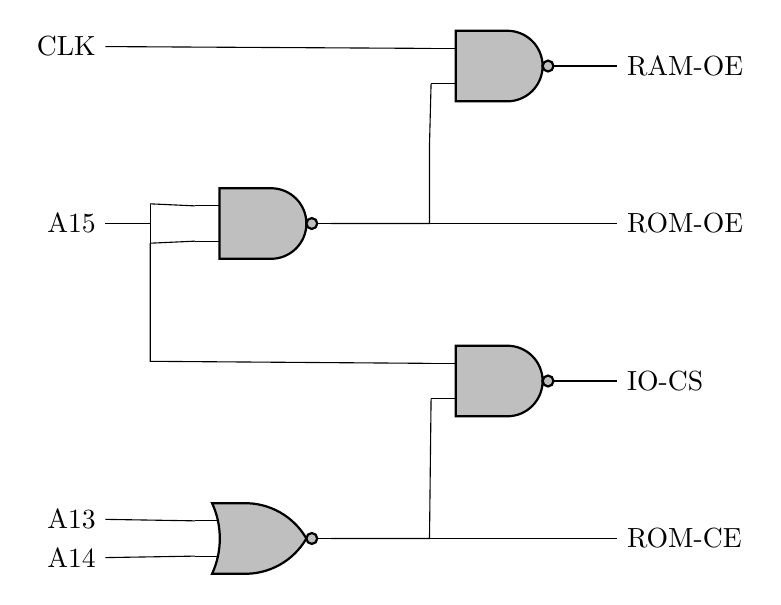
\begin{tikzpicture}
 % Circuit style
\ctikzset{
    logic ports=ieee,
    logic ports/scale=0.8,
    logic ports/fill=lightgray
}
 
% Logic ports
\node[nand port] (U1A) at (5,0){};
\node[nand port] (U1B) at (2,-2){};
\node[nand port] (U1C) at (5,-4){};
\node[nor port] (U2A) at (2,-6){};

\node[left](CLK) at (0,0.25){CLK};
\node[left](A15) at (0,-2){A15};
\node[left](A13) at (0,-5.75){A13};
\node[left](A14) at (0,-6.25){A14};
\node[right](RAM-OE) at (6.5,0){RAM-OE};
\node[right](ROM-OE) at (6.5,-2){ROM-OE};
\node[right](IO-CS) at (6.5,-4){IO-CS};
\node[right](ROM-CE) at (6.5,-6){ROM-CE};

\draw (CLK) -- (U1A.in 1);
\draw (A15) -- ++(1,0)node(A15IN){};
\draw (A15IN) ++(0,0.25) -- +(0,-0.5);
\draw (A15IN) ++(0,0.25) -- (U1B.in 1);
\draw (A15IN) ++(0,-0.25) -- (U1B.in 2);
\draw (A15IN) ++(0,-0.25) -- ++(0,-1.5) -- (U1C.in 1);
\draw (U1B.out) -- ++(1.25,0) -- ++(0,1) -- (U1A.in 2);
\draw (U1B.out) -- (ROM-OE);
\draw (A13) -- (U2A.in 1);
\draw (A14) -- (U2A.in 2);
\draw (U2A.out) -- ++(1.25,0) -- (U1C.in 2);
\draw (U1C.out) -- (IO-CS);
\draw (U1A.out) -- (RAM-OE);
\draw (U2A.out) -- (ROM-CE);
\end{tikzpicture}
\end{center}



\begin{table}[H]
\begin{adjustbox}{width=0.2\textwidth,center=1\textwidth}
\begin{tabular}{|llll|}
\hline

\multicolumn{1}{|l|}
{\textbf{A15}}&\multicolumn{1}{l|}{\textbf{A14}}&\multicolumn{1}{l|}{\textbf{A13}}&\multicolumn{1}{l|}{\textbf{}}\\ \hline

\multicolumn{1}{|l|}{0}&\multicolumn{1}{l|}{X}&\multicolumn{1}{l|}{X}&\multicolumn{1}{l|}{\textbf{RAM}}\\ \hline

\multicolumn{1}{|l|}{1}&\multicolumn{1}{l|}{0}&\multicolumn{1}{l|}{0}&\multicolumn{1}{l|}{\textbf{I/O}}\\ \hline

\multicolumn{1}{|l|}{1}&\multicolumn{1}{l|}{0}&\multicolumn{1}{l|}{1}&\multicolumn{1}{l|}{\textbf{ROM}}\\ \hline

\multicolumn{1}{|l|}{1}&\multicolumn{1}{l|}{1}&\multicolumn{1}{l|}{0}&\multicolumn{1}{l|}{\textbf{ROM}}\\ \hline

\multicolumn{1}{|l|}{1}&\multicolumn{1}{l|}{1}&\multicolumn{1}{l|}{1}&\multicolumn{1}{l|}{\textbf{ROM}}\\ \hline

\end{tabular}
\end{adjustbox}
\end{table}


\pagebreak

\subsection{SPI bus}
Serial Peripheral Interface (SPI) is a common way for low speed serial connections between devices.\\

\subsubsection{SPI bus connections}

The typical SPI bus needs 4 wires, 2 for data, one for clock and one for chip select. The lack of an official standard means that the names for the lines can be one of many ‘standards’\\

In most documentation you will see once device called ‘Master’ and the other as ‘Slave’. You will also see it documented as ‘Controller’ and ‘Peripheral’\\

The data from the Controller to the Peripheral can be marked as any one of:\\

* MOSI - Master Out Slave In.\\
* SIMO - Slave in Master out.\\
* SDI - Serial Data In.\\

The data from the Peripheral to the Controller can be marked as any one of:\\

* MISO - Master In Salve Out.\\
* SOMI - Slave Out Master In.\\
* SDO - Serial Data Out.\\

The clock line is mark as any of:\\

* CLK\\
* SCK\\
* SCLK\\
* SCL\\
* CLOCK\\

\pagebreak
The Chip Select can be marked as any one of:\\

* SS\\
* CS\\
* CSN\\
* CE\\

\Note{The Chip Select line is active low, often written with a bar over the name.}


\subsubsection{SPI Modes}
SPI can be used in one of four modes, each mode is just a difference in the clock phase and when data is latched by the SPI device.\\

\textbf{Mode 0} the clock is idle low, and the data is latched on the rising edge of the clock.\\
\textbf{Mode 1} the clock is idle low, and the data is latched on the falling edge of the clock.\\
\textbf{Mode 2} the clock is idle high, and the data is latched on the falling edge of the clock.\\
\textbf{Mode 3} the clock is idle high, and the data is latched on the rising edge of the clock.\\

\pagebreak

\subsection{Display}
The Display is made up of six seven segment display modules, each module is driven by a 74HC595 shift register chip.\\

Each shift register chip will pass data along to the next shift register one bit at a time when the clock changes.\\

By selecting the display we can just sending 6 bytes on the SPI bus the display will be updated.\\

The ROM function will take a byte and "decode" it to turn on/off the right segments to display the byte.


\subsection{SD Card}
The SPI bus give access to the SD Card.

An SD Card runs in Mode 0.

An SD card runs at 3.3V and so the SD card board has a 5V to 3.3V level shiftier chip.


\subsection{Keypad}
The keypad is setup as a row and column of wires, a push button at the intersection of each row and column.\\

By setting a voltage on a given row we can then check if any assorted column is being pressed.\\

The Scan keypad function in the ROM will check every button in a fraction of a second.\\

\pagebreak

\subsection{Schematic}
\begin{center}
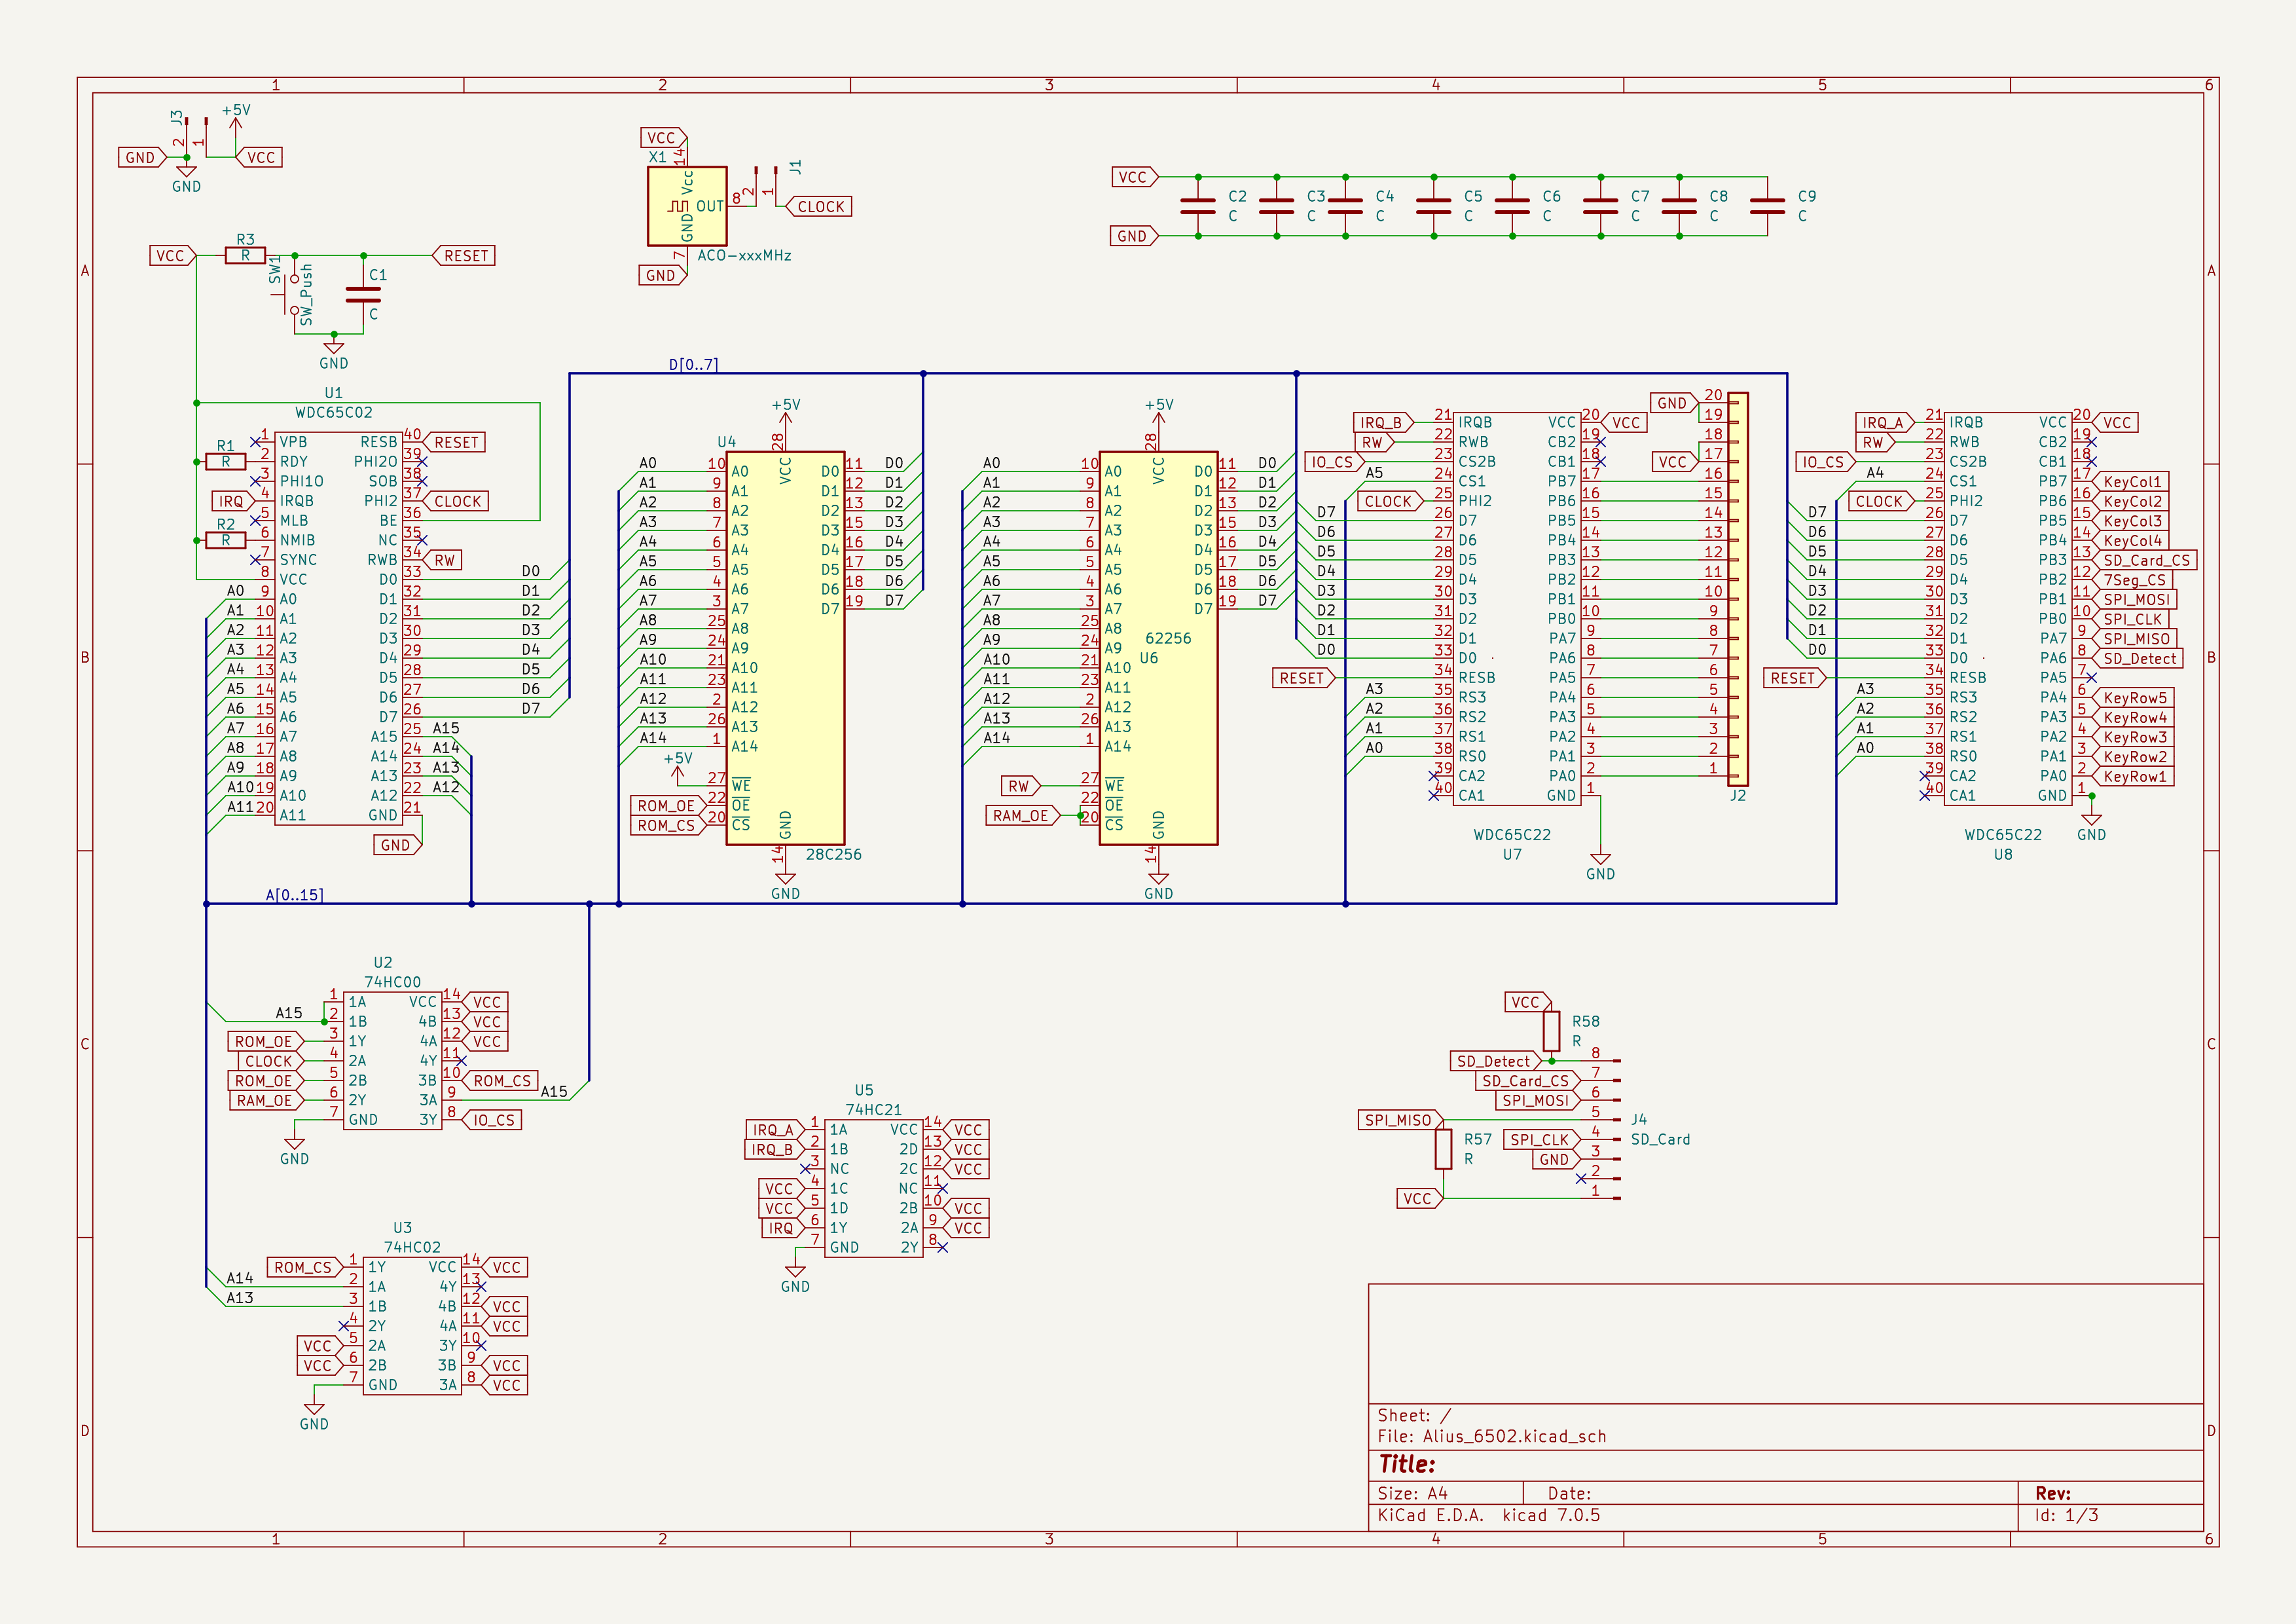
\includegraphics[angle=90,origin=c, width=14.1cm]{Compute.PNG}
\end{center}

\pagebreak

\begin{center}
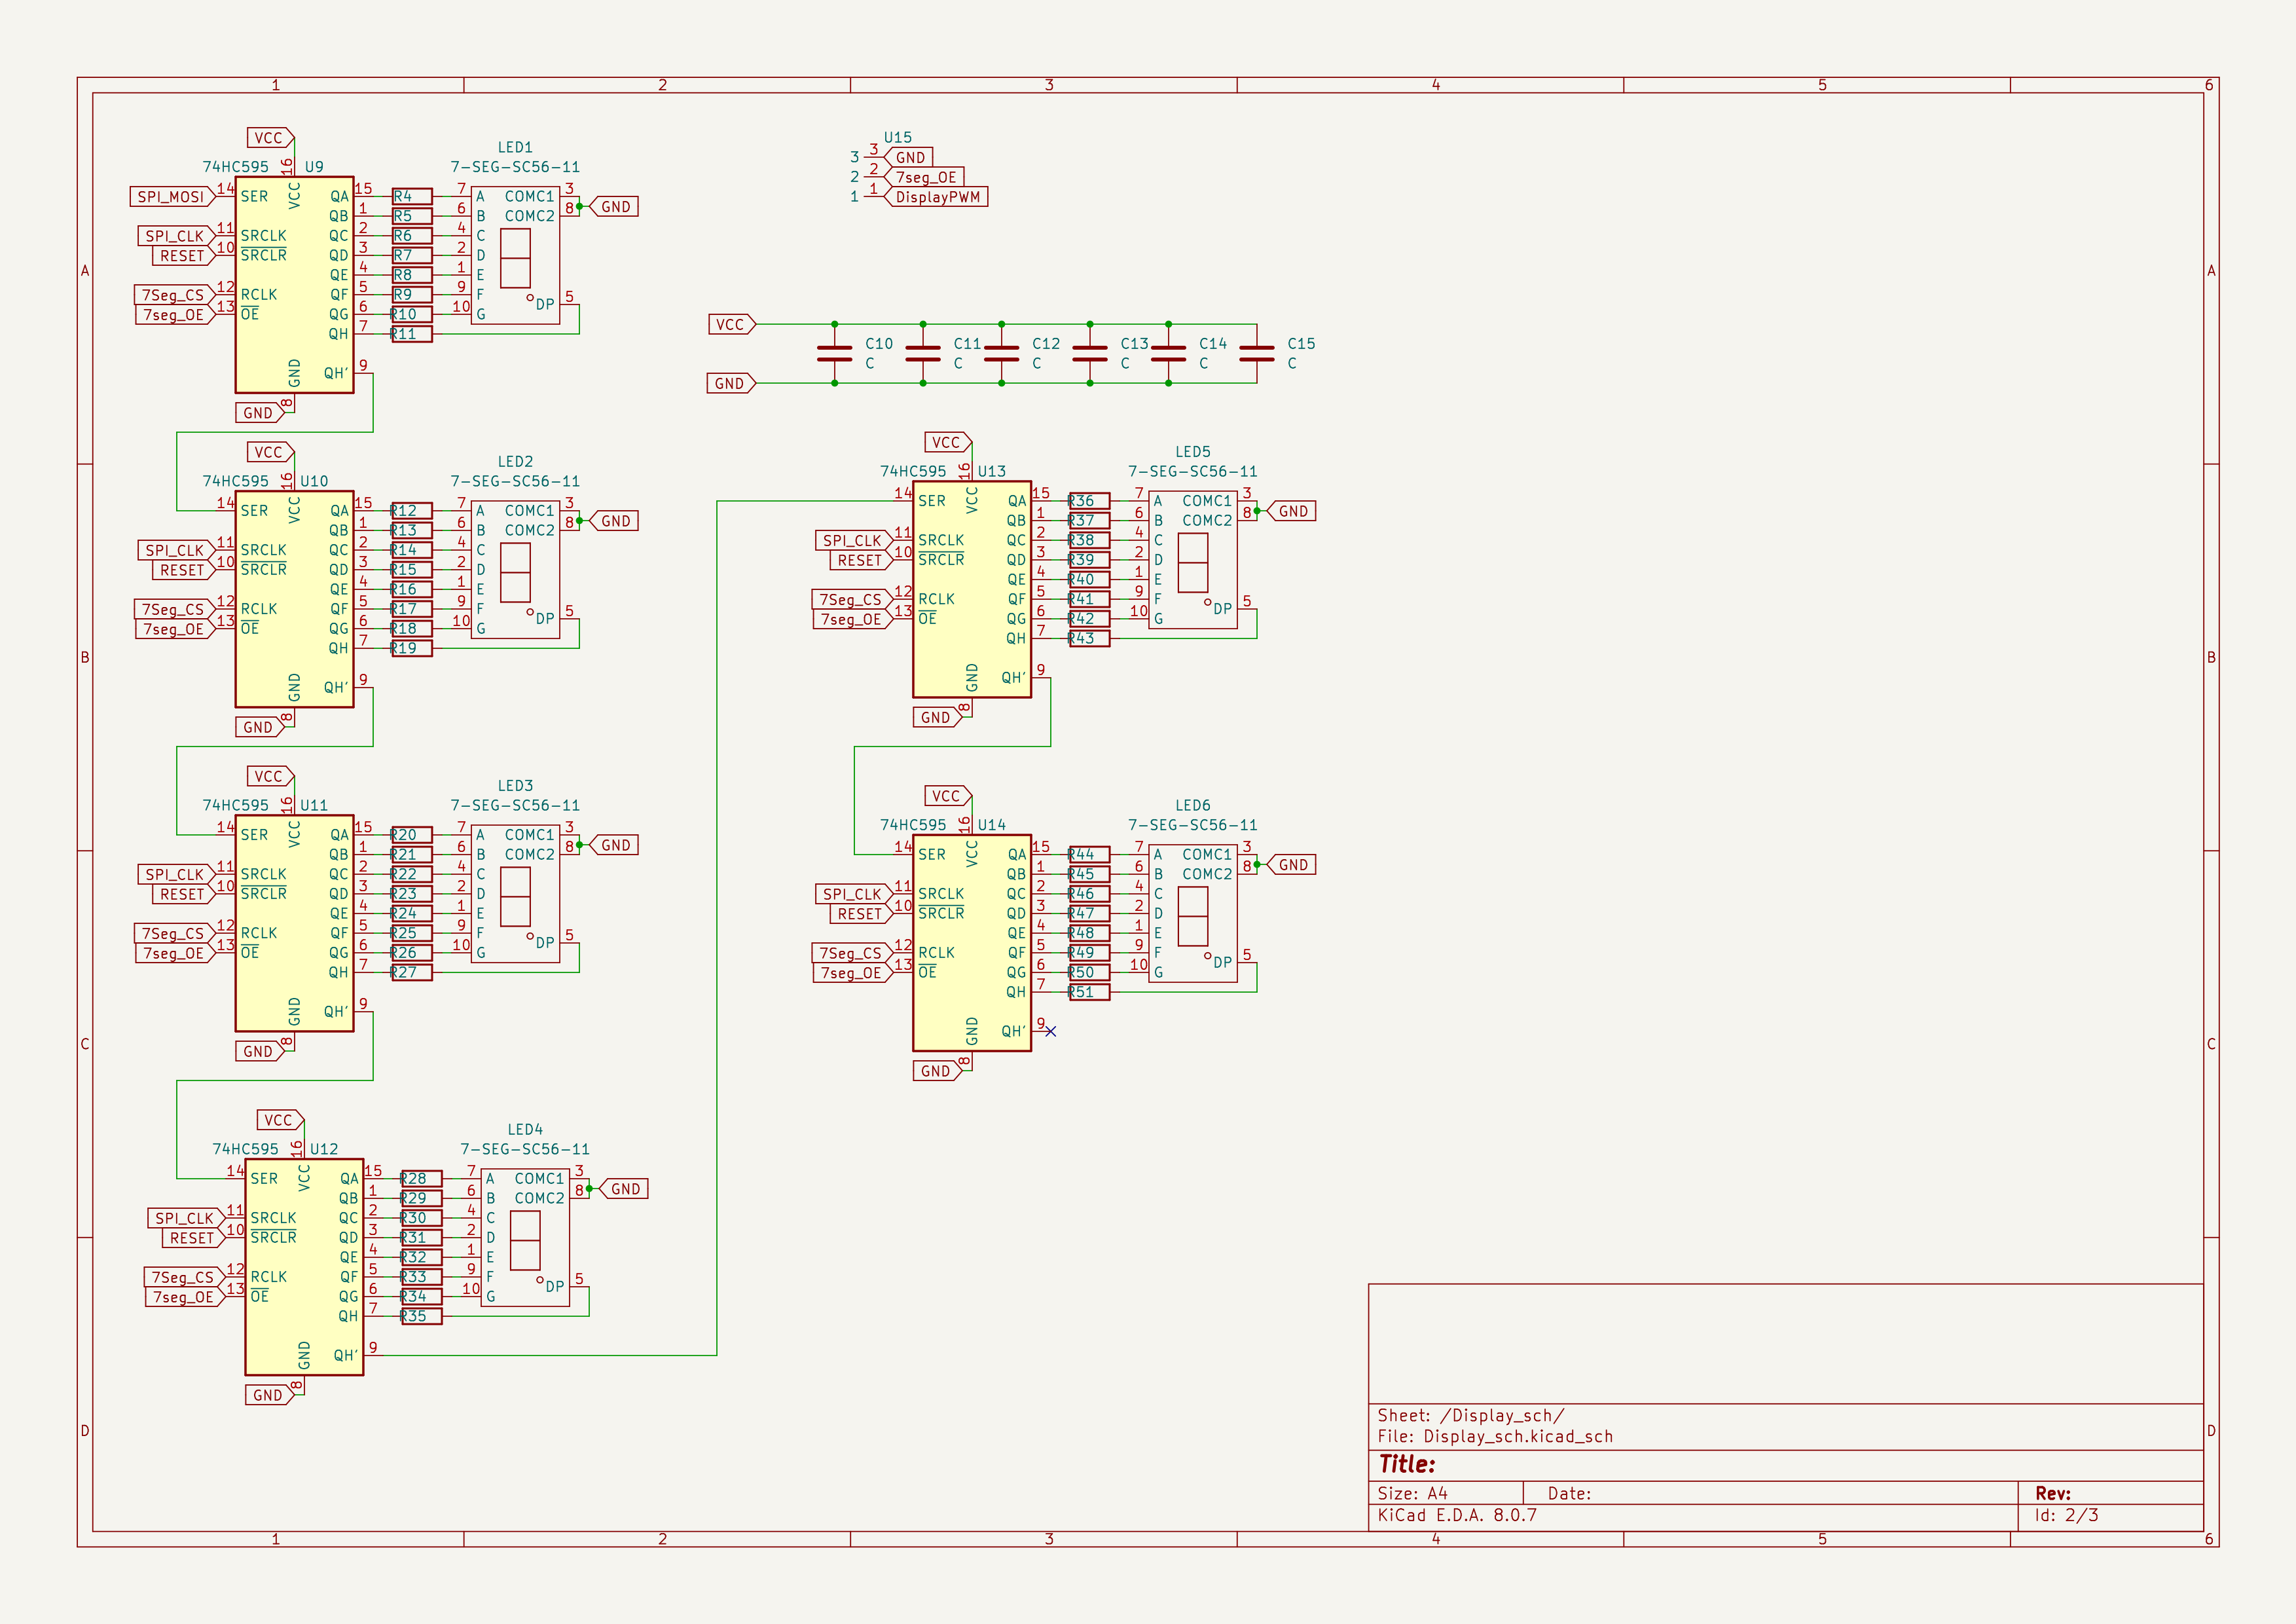
\includegraphics[angle=90,origin=c, width=14.1cm]{Display.PNG}
\end{center}

\pagebreak

\begin{center}
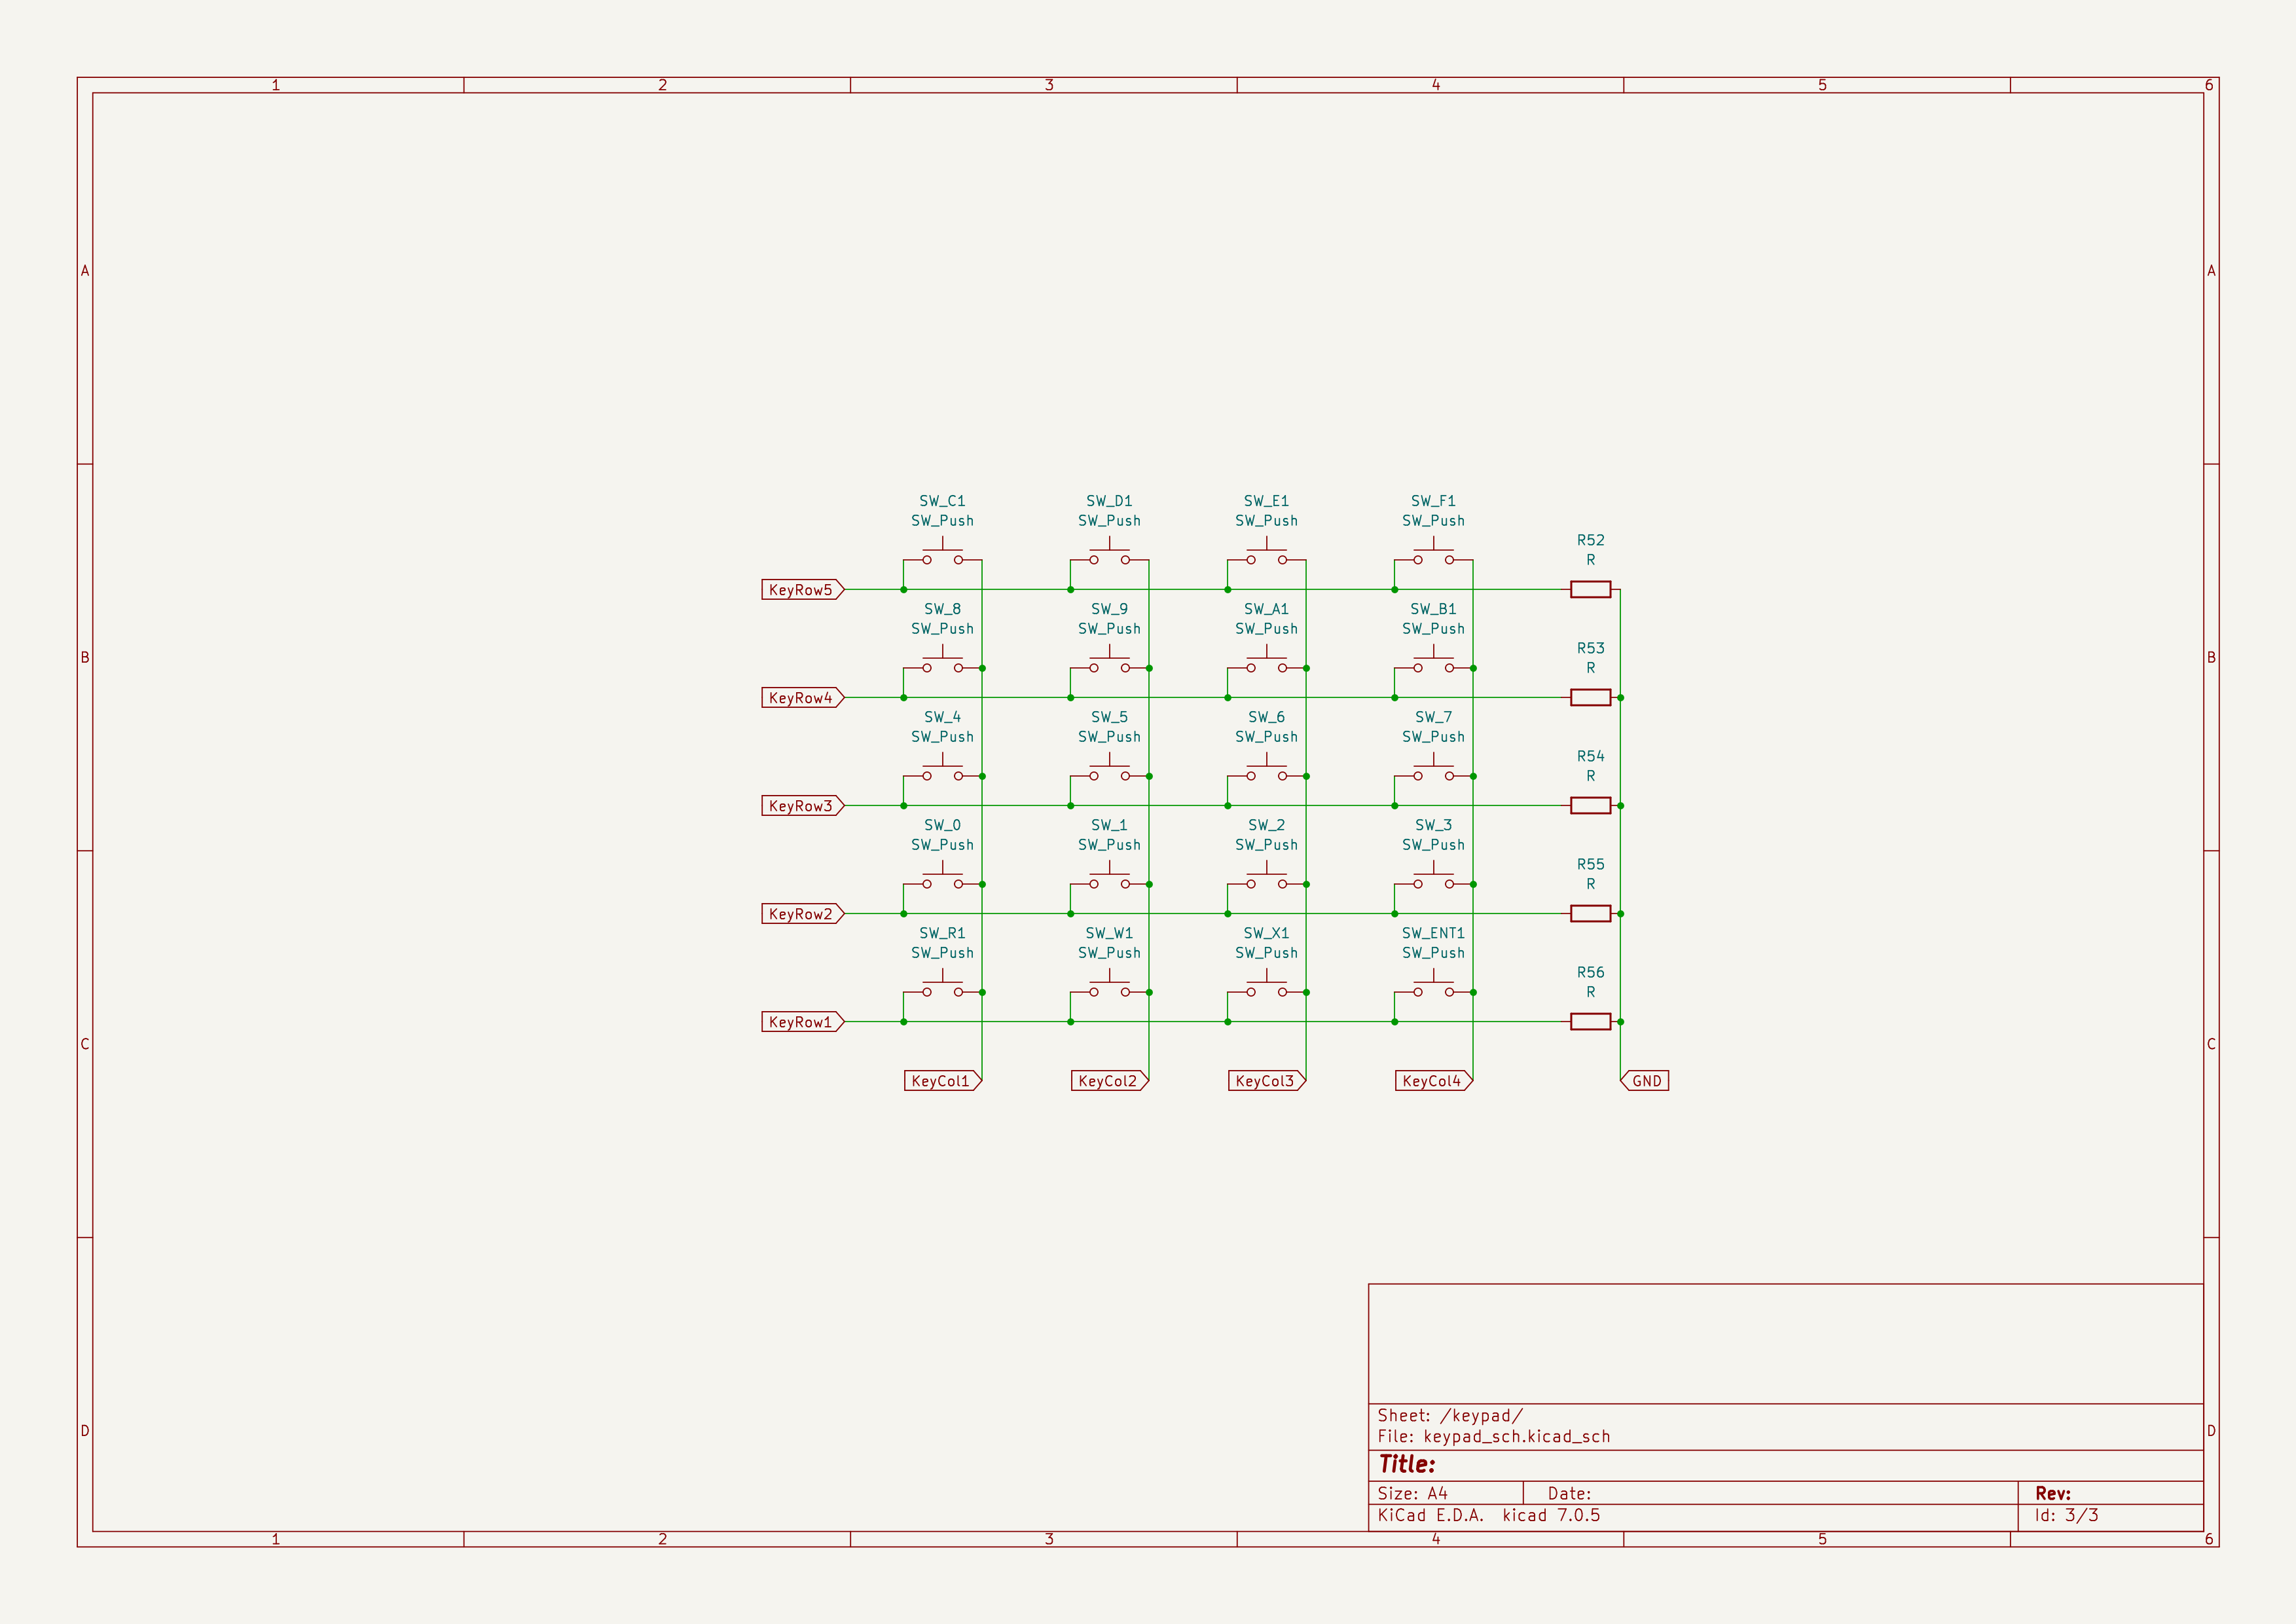
\includegraphics[angle=90,origin=c, width=14.1cm]{Keypad.PNG}
\end{center}

\pagebreak

\section{Building The System}
The Alius 6502 has two different form factors.  The "Wide Board" is best for experiments and the "Stacked Board" makes a good base for a handheld system.\\
\\
NOTE: The two form factors are fully software compatible.\\

\begin{center}
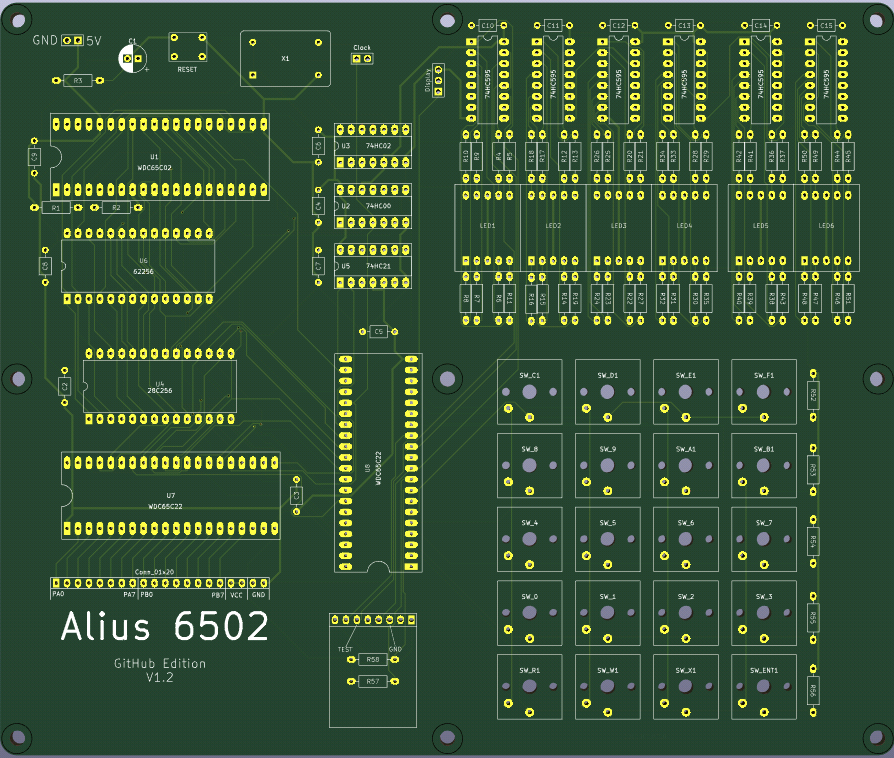
\includegraphics[width=14cm]{Wide_Board.PNG}

Wide Board
\end{center}
\pagebreak

\begin{center}
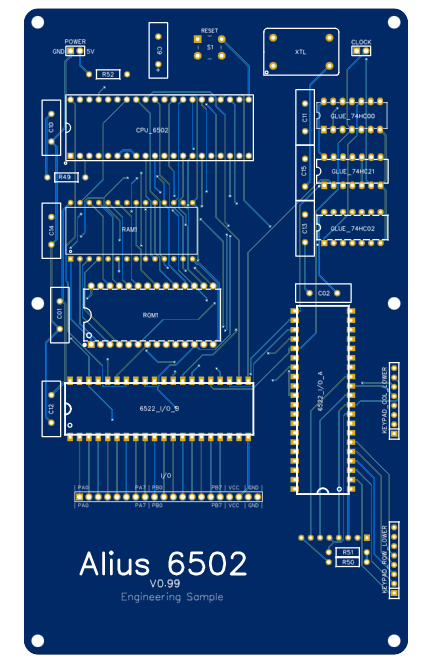
\includegraphics[angle=-90,width=13.5cm]{Bottom_Board.PNG}

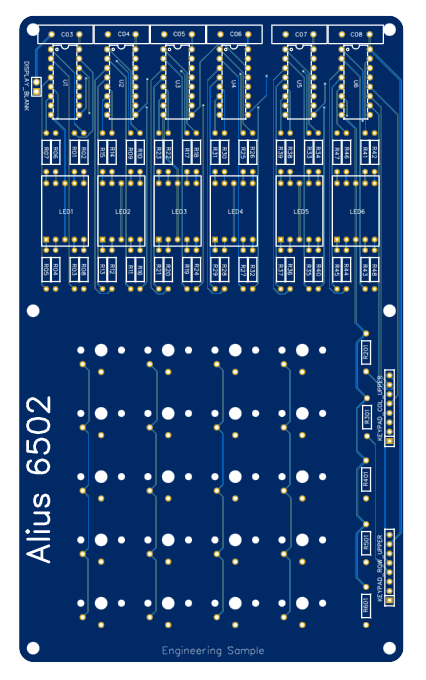
\includegraphics[angle=-90,width=13.5cm]{Top_Board.PNG}

Stacked Board
\end{center}

\pagebreak

\subsection{Parts List}

\begin{table}[H]
\begin{adjustbox}{width=0.9\textwidth,center=1\textwidth}
\begin{tabular}{|lll|}
\hline
\multicolumn{3}{|c|}{\textbf{Alius Parts List}}\\ \hline

\multicolumn{1}{|l|}
{\textbf{QTY}}&\multicolumn{1}{l|}{\textbf{Part}}&\multicolumn{1}{l|}{\textbf{Description}}\\ \hline

\multicolumn{1}{|l|}{1 or 2}&\multicolumn{1}{l|}{Printed Circuit Board(s)}&\multicolumn{1}{l|}{Two boards for the stacked design}\\ \hline

\multicolumn{1}{|l|}{1}&\multicolumn{1}{l|}{1MHz Crystal}&\multicolumn{1}{l|}{}\\ \hline

\multicolumn{1}{|l|}{1}&\multicolumn{1}{l|}{74HC02N}&\multicolumn{1}{l|}{Quad NOR Gate}\\ \hline

\multicolumn{1}{|l|}{1}&\multicolumn{1}{l|}{74HC00N}&\multicolumn{1}{l|}{Quad NAND Gate}\\ \hline

\multicolumn{1}{|l|}{1}&\multicolumn{1}{l|}{74HC21N}&\multicolumn{1}{l|}{Dual 4-Input AND Gate}\\ \hline

\multicolumn{1}{|l|}{1}&\multicolumn{1}{l|}{W65C02S}&\multicolumn{1}{l|}{Main 6502 CPU}\\ \hline

\multicolumn{1}{|l|}{2}&\multicolumn{1}{l|}{WDC65C22}&\multicolumn{1}{l|}{6522 - VIA I/O}\\ \hline

\multicolumn{1}{|l|}{6}&\multicolumn{1}{l|}{74HC595N}&\multicolumn{1}{l|}{Shift register}\\ \hline

\multicolumn{1}{|l|}{6}&\multicolumn{1}{l|}{SC56-11/5011AS}&\multicolumn{1}{l|}{Seven segment red LED}\\ \hline

\multicolumn{1}{|l|}{1}&\multicolumn{1}{l|}{AT28C256}&\multicolumn{1}{l|}{32KB EEPROM}\\ \hline

\multicolumn{1}{|l|}{1}&\multicolumn{1}{l|}{62256P}&\multicolumn{1}{l|}{32KB static RAM}\\ \hline

\multicolumn{1}{|l|}{57}&\multicolumn{1}{l|}{1K$\Omega$ resistor}&\multicolumn{1}{l|}{}\\ \hline

\multicolumn{1}{|l|}{1}&\multicolumn{1}{l|}{10$\mu$f capacitor}&\multicolumn{1}{l|}{}\\ \hline

\multicolumn{1}{|l|}{14}&\multicolumn{1}{l|}{0.1$\mu$f capacitor}&\multicolumn{1}{l|}{}\\ \hline

\multicolumn{1}{|l|}{2}&\multicolumn{1}{l|}{2 pin header}&\multicolumn{1}{l|}{Used for power and clock}\\ \hline

\multicolumn{1}{|l|}{1}&\multicolumn{1}{l|}{3 pin header}&\multicolumn{1}{l|}{Used for display}\\ \hline

\multicolumn{1}{|l|}{1}&\multicolumn{1}{l|}{8 pin header}&\multicolumn{1}{l|}{for SD Card}\\ \hline

\multicolumn{1}{|l|}{1}&\multicolumn{1}{l|}{SD Card module}&\multicolumn{1}{l|}{Adafruit board}\\ \hline

\multicolumn{1}{|l|}{1}&\multicolumn{1}{l|}{Reset switch}&\multicolumn{1}{l|}{}\\ \hline

\multicolumn{1}{|l|}{1}&\multicolumn{1}{l|}{28 pin ZIF socket}&\multicolumn{1}{l|}{ZIF for ROM chip}\\ \hline

\multicolumn{1}{|l|}{20}&\multicolumn{1}{l|}{Kailh Choc switch}&\multicolumn{1}{l|}{}\\ \hline

\multicolumn{1}{|l|}{20}&\multicolumn{1}{l|}{Kailh Choc key cap}&\multicolumn{1}{l|}{}\\ \hline

\multicolumn{3}{|c|}{\textbf{Extra parts for Stacked design}}\\ \hline

\multicolumn{1}{|l|}{2}&\multicolumn{1}{l|}{8 pin header male}&\multicolumn{1}{l|}{}\\ \hline

\multicolumn{1}{|l|}{2}&\multicolumn{1}{l|}{8 pin header female}&\multicolumn{1}{l|}{}\\ \hline

\multicolumn{1}{|l|}{6}&\multicolumn{1}{l|}{M3 standoff}&\multicolumn{1}{l|}{}\\ \hline

\multicolumn{1}{|l|}{12}&\multicolumn{1}{l|}{M3 bolt}&\multicolumn{1}{l|}{}\\ \hline

\end{tabular}
\end{adjustbox}
\end{table}
\Note{Part numbers on chips will normally have letters or numbers before or after the listed part number. For example the "62256" might be marked as "MH62256LP-15"}
\clearpage

\subsection{Tools}
Some tools are nice to have and other tools are a hard requirement, this list is in order of importance.

\subsection{Soldering iron}
\subsection{Solder Remover}
\subsection{Side cutters}
\subsection{Screw Driver}
\subsection{Isopropyl Alcohol}
\subsection{Helping Hands}
\subsection{Multimeter}
\subsection{Magnifying Glass}
\subsection{Variable Power Supply}
\subsection{Oscilloscope}

\pagebreak

\subsection{Construction}
It is recommended that you start by checking you have all the parts listed above and ensure you can identify each part. Use of chip sockets will make any repair and changes easier.\\
\\
The order of steps below has been tested as the best work flow, it also allows for testing during the construction.\\
\\
For components with a large number of pins a good method of soldering them is to solder one pin at each corner to ensure correct fit before soldering all the pins.\\
\\
Depending on your soldering skills and pace of work, the full construction will take 3 to 5 hours.\\
\\
The project build is split into three sections and you can use this as a sensible way to break the project up over a few days.
\\

\pagebreak
\begin{center}
\textbf{Core Compute}
\end{center}
In this section we will build and test the core of the computer.\\
\\
\textbf{Step 1}\\
Install in 3 x 1K$\Omega$ resistors, marked on the board as R1, R2 and R3.\\
\\
\textbf{Step 2}\\
Install reset switch S1.\\
\\
\textbf{Step 3}\\
Install chip sockets for 65C02 CPU, 62256 RAM, 2 x 65C22 I/O chips, 74HC00, 74HC02, 74HC21\\
\\
\textbf{Step 4}\\
Install the ZIF socket for the ROM. This should be mounted to have the lever on the right hand side of the socket.\\
\Note{Pin one of the chip is on the left side of the board, the lever is on thre right for easy access.}\\
\\
\textbf{Step 5}\\
Install capacitor C1
\Note{This is a 10$\mu$f tantalum capacitor, the polarity is marked on the board and on the part.}\\
\\
\textbf{Step 6}\\
Install 8 x 0.1$\mu$f capacitors, C2, C3, C4, C5, C6, C7, C8, C9.\\
\\
\textbf{Step 7}\\
Install 1MHz crystal - marked as X1.\\
The polarity is marked by a dot on the board and one corner of the crystal can is not as rounded as the others.\\
\\
\textbf{Step 8}\\
Install the 2 pin jumper for the clock.\\
\\
\pagebreak

\textbf{Step 9}\\
Install the 8 pin header for the SD Card.\\
\Note{Do not install the whole SD Card board at this point.}\\
\\
\textbf{Step 10}\\
Install a two pin header as power connector.\\
\\
\textbf{Step 11}\\
Insert chips.\\
65C02 CPU, 62256 RAM, 2 x 65C22 I/O chips, 74HC02, 74HC00, 74HC21.\\
\\
\textbf{Step 12}\\
Setup a test LED across SD Card I/O pins marked "Test" and "GND".\\
\\
\textbf{Step 13}\\
Flash the ROM chip with test ROM.\\
\\
\textbf{Step 14}\\
Power up, press reset button, and test.\\
\\
If this stage has all worked correctly you should have the LED blinking about once per second.
\Note{If you do not have a blinking LED then read up on fault finding before proceeding.}
\\
\pagebreak

\begin{center}
\textbf{The Display}
\end{center}
In this section we will build and test the seven segment display.\\
\\
\textbf{Step 15}\\
Install the 48 x 1K$\Omega$ resistors, R4 -> R51\\
\\
\textbf{Step 16}\\
Install 6 x seven segment modules LED1 - > LED6.\\
Be careful to get the polarity correct, the decimal point on the display module is at the bottom right corner.\\
\\
\textbf{Step 17}\\
Install sockets for chips U1 -> U6.\\
\\
\textbf{Step 18}\\
Install 6 x 0.1$\mu$f capacitors C10 -> C15\\
\\
\textbf{Step 19}\\
Install the 3 pin jumper for Display\_Blank.\\
The jumper should be in the upper position.
\Note{If you have the "Wide" design then skip to step 23}\\
\\
\textbf{Step 20} - "Stacked" design only\\
Install the 8 pin male headers on the lower board.\\
\\
\textbf{Step 21} - "Stacked" design only\\
Screw on the 6 x stand offs to the lower board.\\
\\
\textbf{Step 22} - "Stacked" design only\\
Stack the two boards and screw together to correctly position the female headers before soldering.\\
\pagebreak

\textbf{Step 23}\\
Power on and test that all segments of the display light up one by one.
\\
\Note{If you do not have each segment light up then read up on fault finding before proceeding.}
\\
\pagebreak
\begin{center}
\textbf{The Keypad}
\end{center}
In this section we will build the keypad and install the SDcard module.\\
\\
\textbf{Step 24}\\
Install  5 x 1K$\Omega$ resistors, R52, R53, R54, R55, R56\\
\\
\textbf{Step 25}\\
Install the 20 x key switches.\\
\\
\textbf{Step 26}\\
Label the 20 x key caps.\\
\\
\textbf{Step 27}\\
Install the 20 x key caps.\\
\\
\begin{center}
\textbf{The SD Card}
\end{center}
\textbf{Step 28}\\
Install 2 x 1k$\Omega$ resisters R57, R58\\
\\
\textbf{Step 29}\\
Install SD Card board.\\
\\
\textbf{Step 30}\\
Flash the ROM chip with Monitor ROM.\\
\\
\textbf{Step 31}\\
Power up and test.\\

\pagebreak
\subsection{Flashing the ROM}
TL866 II Plus EEPROM Programmer


\pagebreak

\subsection{Fault Finding}
Any electronics project comes with the need for some fault finding. Having everything work first time is not guaranteed. In this section we will look at the most common things to check for issues.

\subsubsection{Check Power}
One of the more frustrating faults is when nothing at all happens.\\
Check for 5V of power on the board. A good test point is the right end of the expansion header. (VCC/GND)\\
\\
If you don't detect 5V then check the power is working. Also check what amperage is being drawn by the board, under 200mA is expected.\\
\\
A high power draw is a sign of a short circuit.\\

\subsubsection{Check Soldering}
The system has in the range of 500 solder joints and most of them are critical to having the system work. A visual inspection under good lighting will find many issues.\\
\\
Look for joints that are missing, joints that have bridged to a next door connections.\\

Removing excessive solder is best done with solder wick, which lets you draw off some solder from the joint.

\subsubsection{Check chips}
It is important that you have the correct chips in the right places, but also inserted in the correct orientation.\\

Bent pins can also happen, you can often straighten pins with tweezers. Just be aware that the pin will never be as strong and might bend again.
\\
\subsubsection{Check jumpers}
The clock jumper is essential to correct operation, and the Display\_Blank jumper is needed to have the display work correctly.\\

\pagebreak
\section{Glossary}
\textbf{CMOS} - Complementary Metal–Oxide–Semiconductor. This is a type of microchip construction.\\
\\
\textbf{CPU} - Central Processing Unit. This is the main chip in a computer and it is where all the math and logic is processed. \\
\\
\textbf{EEPROM} - Electrically Erasable Programmable Read-Only Memory. This is a chip that can hold data that is not lost when power is removed (non-volatile) but can be reprogrammed as required.\\
\\
\textbf{FAT32} - FAT stands for File Allocation Table, FAT32 is a version of the FAT file system created by Microsoft in 1995 and has become a standard for use with SD Cards.\\
\\
\textbf{I/O} - Input/Output. This is the way to get data into and out of a computer.\\
\\
\textbf{IRQ} - Interrupt Request. This is a system in which external hardware can request that the CPU stops running the current code and runs special interrupt handling code.\\
\\
\textbf{LBA} - Logical Block Addressing. This is a common way of addressing which sector or block of data to access on a file system.\\
\\
\textbf{LED} - Light Emitting Diode. A semiconductor device that emits light. \\
\\
\textbf{LSB} - Least Significant Bit or Least Significant Byte. The LSB is sometimes referred to as the low-order bit or right-most bit.\\
\\
\textbf{MHz} - Megahertz. Hertz is a measure of cycles per second, 1 Megahertz is one million cycles per second.\\
\\
\textbf{MOS} - MOS is short for Metal Oxide Semiconductor, but also can relate to MOS Technology, Inc. who are most well known for designing the 6502 CPU.\\
\\
\textbf{MSB} - Most Significant Bit or Most Significant Byte. The MSB is sometimes referred to as the high-order bit or left-most bit.\\
\\
\pagebreak
\\
\textbf{RAM} - Random Access Memory. This is a type of memory that allows data to be accessed in any order and allows for the change of a single byte.\\
\\
\textbf{ROM} - Read Only Memory. A type of memory that can't be changed and keeps the data if power is removed.\\
\\
\textbf{SD Card} - Secure Digital Card. A removable card of memory storage that can be electrically erased and reprogrammed. Often used in place of a hard drive in portable electronics.\\
\\
\textbf{SPI} - Serial Peripheral Interface. A communication interface specification used for simple data interfaces.\\
\\
\textbf{ZIF} - Zero Insertion Force. A special type of chip socket that allows easy insertion and removal of a computer chip. Often used for a ROM chip to allow for easy upgrades.\\

\end{document}




